\chapter{Teoria das Linguagens Regulares}\label{cap:LinguagemRegulares}

% Uma teoria matemática não deve ser considerada completa até que a tenhamos feito tão clara que a possamos explicar ao primeiro homem que encontramos na rua. (David Hilbert)

\epigraph{``Se as pessoas não acreditam que a matemática é simples, é só porque eles não percebem o quão complicada a vida é''}{John Von Neumann}

\section{Autômato Finito Determinístico}\label{sec:AFD}

Como explicado em diversas obras tais como \cite{benjaLivro2010, hopcroft2008, linz2006, menezes1998LFA}, os autômatos finitos podem ser separados em dois tipos bem definidos, a saber Autômato Finito Determinístico (AFD) e Autômato Finito Não-determinístico (AFN). Agora este manuscrito inicia o estudo dos AFD apresentando sua forma algébrica equacional.

\begin{definition}[Autômato Finito Determinístico]\label{def:AFD}
	Um AFD é uma estrutura $A = \langle Q, \Sigma, \delta, q_0, F\rangle$ onde: $Q$ é um conjunto finito de estados, $\Sigma$ é um alfabeto, $\delta : Q \times \Sigma \rightarrow Q$ é uma função total (chamada função de transição), $q_0 \in Q$ é um estado destacado (chamado estado inicial) e $F \subseteq Q$ é o conjunto de estados finais\footnote{Em algumas referências também é usado o termo conjunto de estados de aceitação \cite{de2010}.}.
\end{definition}

\begin{example}\label{exe:AFD}
	A estrutura $A = \langle \{q_0, q_1\}, \{a\}, \delta, q_0, \{q_1\} \rangle$ onde a função de transição é definida por: $\delta(q_0, a) = q_1$ e $\delta(q_1, a) = q_0$, é um AFD.
\end{example}

\begin{example}\label{exe:NaoEAFD}
	A estrutura $B = \langle \{q_0, q_1, q_2\}, \{a, b\}, \delta, q_0, \{q_0\} \rangle$ onde a função de transição é definida por:
	\begin{table*}[h]
		\centering
		\begin{tabular}{ccc}
			$\delta(q_0, a) = q_1$ & $\delta(q_1, a) = q_2$ & $\delta(q_2, a) = q_1$\\
			$\delta(q_0, b) = q_1$ & $\delta(q_1, b) = q_2$ & 
		\end{tabular}
	\end{table*}
	
	\noindent não é um AFD, pois $\delta(q_2, b)$ não está definido, e portanto, $\delta$ não é uma função total.
\end{example}

\begin{note}
	Para simplificar a escrita neste manuscrito as siglas AFD e AFN serão usado tanto para designar o singular quanto o plural, ficando a distinção a critério dos conectivos antes de cada sigla.
\end{note}

A função de transição $(\delta)$ pode ser interpretada semanticamente como sendo o programa que o autômato executa, assim uma aplicação qualquer de $\delta$ é uma instrução do programa do autômato, por exemplo, a aplicação $\delta(q, x) = p$ significa que, se o AFD está no estado atual $q$ e o mecanismo de leitura está lendo um $x$, então mude para o estado $p$. 

Uma representação comum para os AFD é baseada no uso de grafos de transição \cite{valdi2020phd}. Em um grafo de transição os vértices irão ser representados por círculos, que neste caso são usados para representar os estados do autômato, isto é, os círculos representam os elementos de $Q$. Cada aresta $(q_i, q_j)$ são rotuladas por $x$ representando assim a transição da forma $\delta(q_i, x) = q_j$. Por fim, os estados finais, isto é, cada $q \in F$ será representado por vértices desenhados como um círculo duplo em vez de um círculo simples e o estado inicial é marcado com uma seta.

\begin{example}\label{exe:AFDA}
	A representação por grafo de transição do AFD descrito no Exemplo \ref{exe:AFD} corresponde a figura a seguir.
	
	\begin{figure}[ht]
		\centering
		\begin{tikzpicture}[>=stealth, shorten >=1pt, node distance=5.0cm, on grid, auto, state/.append style={minimum size=3em}, thick ]
			\node[state, initial]   (A)               {$q_0$};
			\node[state, accepting] (B) [right of=A]  						 {$q_1$};
			
			\path[->] (A) +(-1,0) edge (A)
			
			%Transições:
			%(Partida) edge [tipo da seta] node {simbolo lido} (Destino)
			(A) edge [bend left]  				node {$a$}     		(B)
			(B) edge [bend left]  				node {$a$}     		(A);
		\end{tikzpicture}
		\caption{Representação visual do AFD no Exemplo \ref{exe:AFD}.}
		\label{fig:AFD}
	\end{figure}
\end{example}

\begin{example}\label{exe:AFDS}
	O AFD $S = \langle \{s_0, s_1, s_2\}, \{0,1\}, \delta, s_0, \emptyset \rangle$ onde a função de transição é definida como sendo: $\delta(s_0, 0) = s_1, \delta(s_1, 0) = s_2, \delta(s_2, 0) = s_1, \delta(s_0, 1) = s_2, \delta(s_1, 1) = s_1$ e $\delta(s_2, 1) = s_1$, é um AFD e pode ser representado pela Figura \ref{fig:AFD2} a seguir.
	
	\begin{figure}[h]
		\centering
		\begin{tikzpicture}[>=stealth, shorten >=1pt, node distance=2.5cm, on grid, auto, state/.append style={minimum size=3em}, thick ]
			\node[state, initial]   			(A)               {$s_0$};
			\node[]		  						(C) [right of=A]  {};
			\node[state] 						(B) [above of=C]  {$s_1$};
			\node[state] 						(D) [below of=C]  {$s_2$};
			
			\path[->] (A) +(-1,0) edge (A)
			
			%Transições:
			%(Partida) edge [tipo da seta] node {simbolo lido} (Destino)
			(B) edge [loop right]               node {$1$}           ( )
			(A) edge			  				node {$0$}     		 (B)
			(A) edge			  				node {$1$}     		 (D)
			(B) edge [bend left]  				node {$0$}     		 (D)
			(D) edge [bend left]  				node [right] {$0, 1$}(B);
		\end{tikzpicture}
		\caption{Representação visual do AFD $S$ do Exemplo \ref{exe:AFDS}.}
		\label{fig:AFD2}
	\end{figure}
\end{example}

Pode-se agora então estender a função de transição, para que o autômato possa vir a processar palavras, em vez de apenas símbolos individuais. 

\begin{definition}[Função de Transição Estendida]\label{def:DeltaEstendido}
	Seja $A = \langle Q, \Sigma, \delta, q_0, F\rangle$ um AFD a função $\delta$ é estendida para uma função $\widehat{\delta}: Q \times \Sigma^* \rightarrow Q$ usando recursividade como se segue.
	\begin{eqnarray}\label{eq:ExtensaoDaFuncaoTransicaoDelta}
		\widehat{\delta}(q, \lambda)& = & q \\
		\widehat{\delta}(q, wa)& = & \delta(\widehat{\delta}(q, w), a)	
	\end{eqnarray}
	onde $q \in Q, a \in \Sigma$ e $w \in \Sigma^*$.
\end{definition}

A partir da definição de função de transição estendida é definida  a noção de computação para os AFD, tal conceito é formalizado a seguir.

\begin{definition}[Computação em AFD]\label{def:ComputacaoAFD}
	Seja $A = \langle Q, \Sigma, \delta, q_0, F\rangle$ um AFD e seja $w \in \Sigma^*$ uma computação de $w$ em $A$ corresponde a aplicação $\widehat{\delta}(q_0, w)$.
\end{definition}

Note que a definição de computação em AFD pode ser interpretada como sendo a resposta ao seguinte questionamento: ``Em que estado o autômato (ou a máquina) estará após iniciar o processamento no estado inicial e ter lido todos os símbolos da palavra de entrada $w$?''

\begin{example}\label{exe:ComputacaoAFD1}
	Considere o AFD do Exemplo \ref{exe:AFD} e a palavra de entrada $aaaa$ tem-se que a computação desta palavra corresponde a:
	\begin{eqnarray*}
		\widehat{\delta}(q_0, aaaa) & = & \delta(\widehat{\delta}(q_0, aaa), a)\\
		& = & \delta(\delta(\widehat{\delta}(q_0, aa), a), a)\\
		& = & \delta(\delta(\delta(\widehat{\delta}(q_0, a), a), a), a)\\
		& = & \delta(\delta(\delta(\delta(\widehat{\delta}(q_0, \lambda), a), a), a), a)\\
		& = & \delta(\delta(\delta(\delta(q_0, a), a), a), a)\\
		& = & \delta(\delta(\delta(q_1, a), a), a)\\
		& = & \delta(\delta(q_0, a), a)\\
		& = & \delta(q_1, a)\\
		& = & q_0
	\end{eqnarray*}
\end{example}

\begin{example}\label{exe:ComputacaoAFD2}
	Considere o AFD do Exemplo \ref{exe:AFDS} e a palavra de entrada $0101$ tem-se que a computação desta palavra corresponde a:
	\begin{eqnarray*}
		\widehat{\delta}(s_0, 0101) & = & \delta(\widehat{\delta}(s_0, 010), 1)\\
		& = & \delta(\delta(\widehat{\delta}(s_0, 01), 0), 1)\\
		& = & \delta(\delta(\delta(\widehat{\delta}(s_0, 0), 1), 0), 1)\\
		& = & \delta(\delta(\delta(\delta(\widehat{\delta}(s_0, \lambda), 0), 1), 0), 1)\\
		& = & \delta(\delta(\delta(\delta(s_0, 0), 1), 0), 1)\\
		& = & \delta(\delta(\delta(s_1, 1), 0), 1)\\
		& = & \delta(\delta(s_1, 0), 1)\\
		& = & \delta(s_2, 1)\\
		& = & s_1
	\end{eqnarray*}
\end{example}

De pose da definição de computação pode-se formalizar o conceito de reconhecimento (ou aceitação) de palavras nos AFD.

\begin{definition}[Reconhecimento de palavras em AFD]\label{defi:PalavraAceitaPorAFD}
	\cite{benjaLivro2010} Sejam $A = \langle Q, \Sigma, \delta, q_0, F\rangle$ um AFD e seja $w \in \Sigma^*$. A palavra $w$ é dita aceita (reconhece ou computada) por $A$ sempre que $\widehat{\delta}(q_0, w) \in F$ e é rejeitada por $A$ em qualquer outro caso.
\end{definition}

É fácil perceber que $\widehat{\delta}(q_0, w) \in F$ com $w = a_1a_2\cdots a_n$ se, e somente se, existir uma sequência finita de estados $(q_i)_{i \in I}$ tal que $\delta(q_0, a_1) = q_{i_1}, \delta(q_{i_1}, a_2) = q_{i_2}, \cdots, \delta(q_{i_{n-1}}, a_{n}) = q_{i_n}$ com $q_n \in F, I$ sendo uma sequencia de números naturais e $i_1, i_2, i_{n-1}, i_n \in I$. O leitor pode notar que em particular tem-se que $\widehat{\delta}(q_0, \lambda) \in F$ se, e somente se, $q_0 \in F$.

\begin{example}\label{exe:AceiteAFD1}
	Considerando os Exemplos \ref{exe:ComputacaoAFD1} e \ref{exe:ComputacaoAFD2} tem-se que a palavra $aaaa$ não é aceita pelo AFD do Exemplo \ref{exe:ComputacaoAFD1}, uma vez que, $q_0 \notin F$. Já a palavra $0101$ também não é aceita pelo AFD do Exemplo \ref{exe:ComputacaoAFD2}, uma vez que, $s_1 \notin F$, de fato o leitor atento pode notar que o AFD do Exemplo \ref{exe:ComputacaoAFD2} não aceita qualquer palavra de entrada pois $F = \emptyset$.
\end{example}

\begin{remark}
	Note que se um AFD não aceitar qualquer palavra, é diferente de dizer que ele não realiza computação, pois como ja mencionado anteriormente uma computação é apenas a aplicação da função $\widehat{\delta}$, já não aceitar palavras diz respeito ao fato que para toda palavra $w$ tem-se que $\widehat{\delta}(q_0, a) \notin F$, isto é, a computação das palavras não terminam em um estado final do AFD.
\end{remark}

\begin{example}\label{exe:AceiteAFD2}
	Considere o AFD representado pelo grafo de transições da Figura \ref{fig:AFD3} a seguir. Por indução sobre o tamanho das palavras é fácil mostrar que este AFD reconhece palavras as palavras $1(10)^n1$ e $0(01)^n0$ com $n \in \mathbb{N}$.
	
	\begin{figure}[h]
		\centering
		\begin{tikzpicture}[>=stealth, shorten >=1pt, node distance=2.7cm, on grid, auto, state/.append style={minimum size=3em}, thick ]
			\node[state, initial]   			(A)               {$q_0$};
			\node[state] 						(B) [right of=A]  {$q_1$};
			\node[state, accepting]				(C) [above of=B]  {$q_2$};
			\node[state, accepting]				(D) [below of=B]  {$q_3$};
			\node[state] 						(E) [right of=B]  {$q_4$};
			
			\path[->] (A) +(-1,0) edge (A)
			
			%Transições:
			%(Partida) edge [tipo da seta] node {simbolo lido} (Destino)
			(A) edge 				            node {$1$}           (C)
			(A) edge			  				node {$0$}     		 (D)
			(C) edge [bend left]  				node {$1$}     		 (E)
			(C)	edge							node [left] {$0$}	 (B)
			(E) edge [bend left]  				node [right] {$0$} 	 (C)
			(D) edge [bend left]  				node [right] {$0$}	 (E)
			(D)	edge							node [left] {$1$}	 (B)
			(E) edge [bend left]  				node {$1$} 	 		 (D)
			(B) edge [loop left]                node {$0,1$}         ( );
		\end{tikzpicture}
		\caption{Um AFD com dois estados finais.}
		\label{fig:AFD3}
	\end{figure}
\end{example}

Tendo definido precisamente as noções de AFD e de computação em AFD, agora é possível definir formalmente a ideia de linguagem reconhecida (ou computada) por um AFD.

\begin{definition}[Linguagem de um AFD]\label{def:LinguagemAFD}
	Seja $A = \langle Q, \Sigma, \delta, q_0, F\rangle$ um AFD a linguagem reconhecida (ou computada) por $A$, denotada por $\mathcal{L}(A)$, corresponde ao conjunto de todas as palavras aceitas por $A$, formalmente tem-se que:
	\begin{eqnarray}
		\mathcal{L}(A) = \{w \in \Sigma^* \mid \widehat{\delta}(q_0, w) \in F\}
	\end{eqnarray}
\end{definition}

Utilizando a definição acima o leitor deve ser capaz de perceber que se um AFD reconhece uma linguagem $L \subseteq \Sigma^*$, então ele para em estados finais apenas para as palavras $w \in L$. Em outra palavra para mostrar que uma linguagem $L$ é a linguagem de um AFD $A$, deve-se provar que $L = \mathcal{L}(A)$, ou seja, deve-se provar que $w \in L \Longleftrightarrow w \in \mathcal{L}(A)$, em geral quando $L$ é infinito tal prova é por indução.

\begin{example}\label{exe:AFDLinguagem1}
	A seguir você encontrará a prova de que a linguagem $L = \{bba^{2n} \mid n \in \mathbb{N}\}$ é reconhecida pelo AFD $A_1$ na Figura \ref{fig:AFDLinguagem1} a seguir. 
	\begin{figure}[h]
		\centering
		\begin{tikzpicture}[>=stealth, shorten >=1pt, node distance=2.5cm, on grid, auto, state/.append style={minimum size=3em}, thick ]
			\node[state, initial]				(A)               	{$q_0$};
			\node[state] 						(B) [right of=A] 	{$q_1$};
			\node[state, accepting]				(C) [right of=B] 	{$q_2$};
			\node[state]						(D) [below of=C] 	{$q_3$};
			\node[state]						(E)	[right of=C]	{$q_4$};
			\path[->] (A) +(-1,0) edge (A)
			
			%Transições:
			%(Partida) edge [tipo da seta] node {simbolo lido} (Destino)
			(A) edge			  				node {$b$}		 (B)
			(A) edge			  				node {$a$}		 (D)
			(B) edge			  				node {$b$}		 (C)
			(B) edge			  				node {$a$}		 (D)
			(C) edge			  				node {$b$}		 (D)
			(C) edge [bend right] 			  	node {$a$}		 (E)
			(E) edge [bend right] 			  	node {$a$}		 (C)
			(E) edge			  				node {$b$}		 (D)
			(D) edge [loop right] 			  	node {$a,b$}	 ( );
		\end{tikzpicture}
		\caption{AFD $A_1$ que reconhece a linguagem $\{bba^{2n} \mid n \in \mathbb{N}\}$.}
		\label{fig:AFDLinguagem1}
	\end{figure}
	
	\begin{proof}
		$(\Rightarrow)$ Suponha que $w \in L$ assim $w = bba^{2n}$ e por indução sobre o tamanho das palavras tem-se que,
		\begin{itemize}
			\item \textbf{Base da indução}:
			
			Quando $n = 0$ vale que $w = bba^{2\cdot 0}$ e usando a definição do AFD tem-se que, 
			$$\widehat{\delta}(q_0, bba^{2\cdot 0}) = \widehat{\delta}(q_0, bb) = \delta(\widehat{\delta}(q_0, b), b) = \delta(\delta(\widehat{\delta}(q_0, \lambda), b), b) = q_2$$
			como $q_2 \in F$ tem-se que $bb \in \mathcal{L}(A_1)$.
			
			\item \textbf{Hipótese indutiva (HI)}:
			
			Suponha que para todo $n \in \mathbb{N}$ tem-se que $\widehat{\delta}(q_0, bba^{2n}) \in F$, ou seja, $\widehat{\delta}(q_0, bba^{2n}) = q_2$.
			
			\item \textbf{Passo indutivo}:
			
			Dado $w = bba^{2(n+1)}$ tem-se que
			\begin{eqnarray*}
				\widehat{\delta}(q_0, bba^{2(n+1)}) & = & \widehat{\delta}(q_0, bba^{2n + 2})\\
				& = & \widehat{\delta}(q_0, bba^{2n}aa)\\
				& = & \delta(\delta(\widehat{\delta}(q_0, bba^{2n}), a), a)\\
				& \stackrel{\textbf{(HI)}}{=} & \delta(\delta(q_2, a), a)\\
				& = & \delta(q_3, a)\\
				& = & q_2
			\end{eqnarray*} 
			Logo $\widehat{\delta}(q_0, bba^{2n}) \in \mathcal{L}(A_1)$.
		\end{itemize} 
		$(\Leftarrow)$ Suponha que $w \in \mathcal{L}(A_1)$, assim pela definição do AFD $A_1$ tem-se que $\widehat{\delta}(q_0, w) = q_2$, entretanto, pela definição de $\delta$ (ver Figura \ref{fig:AFDLinguagem1}) tem-se que $q_2$ só é acessado pelas transições $\delta(q_1, b)$ e $\delta(q_4, a)$, ou seja, $w = w_1a$ ou $w = w_2b$ com $w_1, w_2 \in \Sigma^*$. Agora analisando cada possibilidade em separado tem-se que: 
		\begin{itemize}
			\item Para realizar o acesso via $q_1$ é necessário obviamente chegar em $q_1$ e isso só é possível a partir da transição $\delta(q_0, b)$, logo o acesso a $q_2$ via $q_1$ só é permitido para palavras com o prefixo $bb$, agora como toda palavra é prefixo de si mesmo isso já garante que $bb \in \mathcal{L}(A_1)$.
			\item Já o acesso via $q_4$ só é permitido pela transição $\delta(q_2, a)$ e como visto no caso anterior tem-se que o estado $q_2$ só pode ser acessado por palavras com prefixo $bb$, note porém, que as transições $\delta(q_2, a) = q_4$ e $\delta(q_4, a) = q_2$ formam um \textit{loop} e assim pode-se concluir que o acesso a $q_2$ via $q_4$ obrigatoriamente é realizado por palavras da forma $bba^{2n}$ com $n \geq 1$.
		\end{itemize}
		Note que a palavra $bb$ pode ser escrita como sendo $bba^0$, portanto, pelas duas análises anteriores pode-se concluir que se $\widehat{\delta}(q_0, w) = q_2$, então $w = bba^{2n}$ com $n \in \mathbb{N}$, logo $w \in L$, completando assim a prova. 
	\end{proof}
\end{example}

\begin{example}
	O AFD $A$ do Exemplo \ref{exe:AFD} reconhece a linguagem $L = \{a^{2n + 1} \mid n \in \mathbb{N}\}$.
	\begin{proof}
		$(\Rightarrow)$ Suponha que $w \in L$ assim $w = a^{2n+1}$, agora por indução sobre o tamanho das palavras tem-se que, 
		
		\begin{itemize}
			\item \textbf{Base da indução}:
			
			Quando $n = 0$ vale a igualdade $w = a^{2\cdot 0+1}$, agora usando a definição do AFD $A$ tem-se que, 
			\begin{eqnarray*}
				\widehat{\delta}(q_0, a^{2\cdot 0+1}) = \widehat{\delta}(q_0, a^{1}) = \delta(\widehat{\delta}(q_0, \lambda), a) = \delta(q_0, a) = q_1
			\end{eqnarray*}
			e como $q_1 \in F$ tem-se que $a^{2\cdot 0+1} \in \mathcal{L}(A)$, ou seja, $w \in \mathcal{L}(A)$.
			
			\item \textbf{Hipótese indutiva (HI)}:
			
			Suponha que para todo $n \in \mathbb{N}$ tem-se que $\widehat{\delta}(q_0, a^{2n+1}) \in F$, ou seja, $\widehat{\delta}(q_0, a^{2n+1}) = q_1$.
			
			\item \textbf{Passo indutivo}:
			
			Dado $w = a^{2(n+1)+1}$ tem-se que,
			
			\begin{eqnarray*}
				\widehat{\delta}(q_0, a^{2(n+1)+1}) & = & \widehat{\delta}(q_0, a^{2n+1+2})\\
				& = & \widehat{\delta}(q_0, a^{2n+1}aa)\\
				& = & \delta(\delta(\widehat{\delta}(q_0, a^{2n+1}), a), a)\\
				& \stackrel{\textbf{(HI)}}{=} & \delta(\delta(q_1, a), a)\\
				& = & \delta(q_0, a)\\
				& = & q_1
			\end{eqnarray*}
		\end{itemize}
		$(\Leftarrow)$ A volta fica como exercício argumentativo ao leitor.
	\end{proof}
\end{example}

Pode-se agora formalizar a primeira das classes de linguagens sendo esta a classe das linguagens regulares, tal classe foi primeiramente definida por Kleene em seu trabalho \cite{kleene1951}, entretanto, em tal ocasião tais linguagens foram chamadas de eventos regulares, como será visto é momentos futuros nesse manuscrito a classe das linguagens regulares é aquela que possui o menor nível complexidade computacional.

\begin{definition}[Linguagens Regulares]\label{def:LinguagensRegulares}
	Uma linguagem $L$ qualquer é dita ser regular se, e somente se, existe um AFD $A$ tal que $L = \mathcal{L}(A)$. A classe de todas as linguagens regulares é denotada por $\mathcal{L}_{Reg}$.
\end{definition}

\section{Autômato Finito Não-determinístico}\label{sec:AFN}

Como explicado por Peter Linz em \cite{linz2006}, um autômato finito não-determinístico, ou simplesmente AFN, é um autômato que se diferencia dos AFD apenas no quesito da função de transição. A diferença consiste no fato de que, enquanto a imagem da função de transição em um AFD é sempre um estado, nos AFN a imagem da  função de transição é um subconjunto de estados, em um sentido moderno da teoria dos autômatos, um AFN seria uma máquina que algumas transições geraria uma superposição de estados \cite{valdi2020phd}. Formalmente um AFN é como se segue.

\begin{definition}[Autômato Finito Não-determinístico]\label{def:AFN}
	Um AFN é uma estrutura $A = \langle Q, \Sigma, \delta_N, q_0, F\rangle$ onde: $Q, \Sigma, q_0$ e $F$ são da mesma forma que na Definição \ref{def:AFD}, já $\delta_N : Q \times \Sigma \rightarrow \wp(Q)$ é uma função total (chamada função de transição não determinística).
\end{definition}

\begin{example}\label{exe:AFN1}
	A estrutura $A = \langle \{q_0, q_1, q_2\}, \{a, b\}, \delta_N, q_0, \{q_0, q_1\}  \rangle$ onde a função $\delta$ é descrita pela Tabela \ref{tab:DeltaAFN1} a seguir é um AFN.
	
	\begin{table}[h]
		\centering
		\begin{tabular}{c|cc}
			\backslashbox{$Q$}{$\Sigma$}	& $a$ & $b$\\ \hline
			$q_0$  & $\{q_1\}$ & $\{q_0\}$\\
			$q_1$  & $\{q_2\}$ & $\{q_0, q_2\}$\\
			$q_2$  & $\{q_2\}$ & $\{q_1\}$\\ \hline
		\end{tabular}
		\caption{Tabela de transição para a função $\delta_N$ do AFN no Exemplo \ref{exe:AFN1}.}
		\label{tab:DeltaAFN1}
	\end{table}
\end{example}

A representação visual de um AFN usando grafos de transição é construída exatamente da mesma forma que a representação de um AFD, a diferença é o fato de poder existir múltiplas arestas rotuladas por um símbolo $a \in \Sigma$ saindo de um vértice $q_i$ e chegando nos vértices $q_j \in X$ onde $X \subseteq Q$ e existe a transição $\delta_N(q_i, a) = X$.

\begin{example}
	O grafo de transição representado na Figura \ref{fig:AFN1} a seguir é uma representação para o AFN do Exemplo \ref{exe:AFN1}.
	
	\begin{figure}[h]
		\centering
		\begin{tikzpicture}[>=stealth, shorten >=1pt, node distance=2.5cm, on grid, auto, state/.append style={minimum size=3em}, thick ]
			\node[state, initial, accepting]	(A)               	{$q_0$};
			\node[state, accepting]				(B) [right of=A] 	{$q_1$};
			\node[state]				        (C) [right of=B] 	{$q_2$};
			\path[->] (A) +(-1,0) edge (A)
			
			%Transições:
			%(Partida) edge [tipo da seta] node {simbolo lido} (Destino)
			(A) edge [bend right]  				node [below] {$a$}		 (B)
			(A) edge [loop above]  				node 		 {$b$}		 ( )
			(B) edge [bend right]  				node [above] {$b$}		 (A)
			(B) edge [bend right]  				node [below] {$a, b$}	 (C)
			(C) edge [bend right] 				node [above] {$b$}		 (B)
			(C) edge [loop above]  				node {$a$}		 		 ( );
		\end{tikzpicture}
		\caption{Grafo de transição do AFN do Exemplo \ref{exe:AFN1}.}
		\label{fig:AFN1}
	\end{figure}
\end{example}

\begin{remark}
	Para as transições da forma $\delta_N(q_0, a) = \emptyset$ tem-se que as mesma não são representadas no grafo de transição de um AFN.
\end{remark}

\begin{note}
	Em muitos texto como por exemplo \cite{benjaLivro2010, linz2006, sipser2010}, as funções de transição não determinísticas são representadas simplesmente por $\delta$, neste texto está sendo usada a notação $\delta_N$ simplesmente para enfatizar a natureza não determinística do autômato na esperança de torna o entendimento mais simples para o leitor.
\end{note}

Como para o caso determinístico a função de transição $\delta_N$ também pode ser estendida para uma função $\widehat{\delta_N}$ usando recursividade como se segue.

\begin{definition}[Transição não-determinística estendida]\label{def:FuncaoDeltaNDEstendida}
	Seja $A = \langle Q, \Sigma, \delta_N, q_0, F\rangle$ um AFN, a função de transição estendida é uma função $\delta_N: Q \times \Sigma^* \rightarrow \wp(Q)$ definida pela seguinte recursão.
	\begin{eqnarray}\label{eq:FuncaoDeltaNDEstendida}
		\widehat{\delta_N}(q, \lambda)& = & \{q\} \\
		\widehat{\delta_N}(q, wa)& = & \bigcup_{q' \in \widehat{\delta_N}(q, w)} \delta_N(q', a)
	\end{eqnarray}
\end{definition}

Como para os AFD a noção de computação em qualquer AFN consiste simplesmente da aplicação da função $\widehat{\delta_N}$ sobre alguma palavra $w \in \Sigma^*$ e um estado $q$. 

\begin{example}\label{exe:ComputacaoAFN}
	Considerando o AFN ilustrado na Figura \ref{fig:AFN1} e a palavra $``abb$'' tem-se que,
	\begin{eqnarray}\label{eq:AFNComptuacao1}
		\widehat{\delta_N}(q_0, abb) & = & \bigcup_{q' \in \widehat{\delta_N}(q_0, ab)} \delta_N(q', b)
	\end{eqnarray}
	e também tem-se que, 
	\begin{eqnarray}\label{eq:AFNComptuacao2}
		\widehat{\delta_N}(q_0, ab) & = & \bigcup_{q'' \in \widehat{\delta_N}(q_0, a)} \delta_N(q'', b)
	\end{eqnarray}
	e
	\begin{eqnarray}\label{eq:AFNComptuacao3}
		\widehat{\delta_N}(q_0, a) & = & \bigcup_{q''' \in \widehat{\delta_N}(q_0, \lambda)} \delta_N(q''', a) \nonumber \\ 
		& = & \bigcup_{q''' \in \{q_0\}} \delta_N(q''', a) \\
		& = & \delta_N(q_0, a) \nonumber \\ 
		& = & \{q_1\} \nonumber
	\end{eqnarray}
	substituindo a Equação (\ref{eq:AFNComptuacao3}) na Equação (\ref{eq:AFNComptuacao2}) tem-se que, 
	\begin{eqnarray}\label{eq:AFNComptuacao4}
		\widehat{\delta_N}(q_0, ab) & = & \{q_0, q_2\}
	\end{eqnarray}
	e finalmente substituindo a Equação (\ref{eq:AFNComptuacao4}) na Equação (\ref{eq:AFNComptuacao1}) tem-se que,
	\begin{eqnarray}
		\widehat{\delta_N}(q_0, aba) & = & \{q_0, q_1\}
	\end{eqnarray}
	ou seja, a computação da palavra $``abb$'' pelo AFN da Figura \ref{fig:AFN1} termina no conjunto de estados $\{q_0, q_1\}$.
\end{example}

Pelo exemplo anterior o leitor mais atento pode ter notado que diferente do caso determinístico, a computação em um AFN não é linear, no sentido de que não existe um único caminho de computação\footnote{Como explicado em \cite{valdi2020phd} um caminho de computação é uma sequência de estados assumidos pela unidade central do autômato durante o processamento de uma palavra de entrada.}, em vez disso, a computação em um AFN pode ser vista como uma árvore em que a união dos estados em cada nível da árvore representa a superposição de estados assumida pela unidade de controle do autômato a cada símbolo consumido (computado ou lido) da palavra $w$, o exemplo a seguir ilustra bem essa ideia de árvore de computação.

\begin{example}\label{exe:ArvoreComputacaoAFN}
	Considerando o AFN ilustrado na Figura \ref{fig:AFN1} e a palavra ``$abab$'' tem-se que o processo de computação para tal palavra poder ser representado pela árvore da Figura \ref{fig:ArvoreComputacaoAFN} a seguir.
	
	\begin{figure}[h]
		\centering
		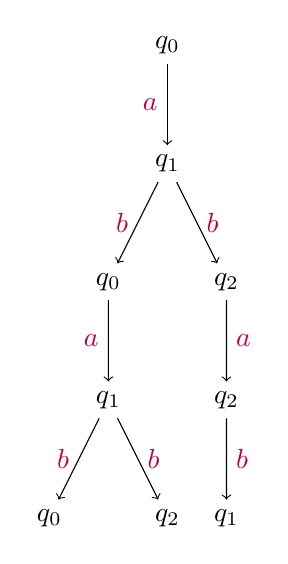
\begin{tikzpicture}
			\node {$q_0$}
			child { node {$q_1$} 
				child {node {$q_0$}
					child {node {$q_1$}
						child {node {$q_0$}
							edge from parent [->] node [left, purple] {$b$}
						}
						child {node {$q_2$}
							edge from parent [->] node [right, purple] {$b$}
						}
						edge from parent [->] node [left, purple] {$a$}
					}
					edge from parent [->] node [left, purple] {$b$}
				}
				child {node {$q_2$}
					child {node {$q_2$}
						child {node {$q_1$}
							edge from parent [->] node [right, purple] {$b$}
						}
						edge from parent [->] node [right, purple] {$a$}
					}
					edge from parent [->] node [right, purple] {$b$}
				}
				edge from parent [->] node [left, purple] {$a$}
			}
			;
		\end{tikzpicture}
		\caption{Árvore de computação da palavra ``$abab$'' no AFN da Figura \ref{fig:AFN1}.}
		\label{fig:ArvoreComputacaoAFN}
	\end{figure}
\end{example}

Pode-se agora apresentar a noção de aceitação (reconhecimento ou computação) de palavras nos AFD.

\begin{definition}[Reconhecimento de palavras em AFN]\label{defi:PalavraAceitaPorAFN}
	Sejam $A = \langle Q, \Sigma, \delta_N, q_0, F\rangle$ um AFN e seja $w \in \Sigma^*$. A palavra $w$ é dita aceita (reconhece ou computada) por $A$ sempre que $\widehat{\delta}(q_0, w) \cap F \neq \emptyset$ e é rejeitada por $A$ em qualquer outro caso.
\end{definition}

Note que a Definição \ref{defi:PalavraAceitaPorAFN} pode ser informalmente interpretada da seguinte forma, uma palavra é aceita por um AFN $A$ se existe pelo menos um caminho de computação para $w$ que termine em um estado final, isto é, pelo menos uma das folhas na árvore de computação deve ser um estado $q \in F$, neste caso $w$ é aceita por $A$.´

\begin{example}\label{exe:AceitacaoEmAFN}
	Considerando o AFN representado pela Figura \ref{fig:AFN2} a seguir,
	
	\begin{figure}[h]
		\centering
		\begin{tikzpicture}[>=stealth, shorten >=1pt, node distance=3.0cm, on grid, auto, state/.append style={minimum size=3em}, thick ]
			\node[state, initial]				(A)               	{$q_0$};
			\node[state, accepting]				(B) [right of=A] 	{$q_1$};
			\node[state]				        (C) [right of=B] 	{$q_2$};
			\node[state]				        (D) [right of=C] 	{$q_3$};
			\path[->] (A) +(-1,0) edge (A)
			
			%Transições:
			%(Partida) edge [tipo da seta] node {simbolo lido} (Destino)
			(A) edge 			 				node [below] {$a$}		 (B)
			(A) edge [loop above]  				node 		 {$a$}		 ( )
			(B) edge 			  				node [above] {$b$}		 (C)
			(C) edge [loop above]  				node 		 {$b$}		 ( )
			(C) edge 			  				node [above] {$b$}		 (D)
			(D) edge [loop above]  				node 		 {$a$}		 ( )
			(D) edge [bend left]  				node [below] {$a$}		 (B);
		\end{tikzpicture}
		\caption{Grafo de transição de um AFN do Exemplo \ref{exe:AceitacaoEmAFN}.}
		\label{fig:AFN2}
	\end{figure}
	
	
	\noindent para as palavras ``$aabbbba$'' e ``$aabb$'' tem-se que: 
	$$\widehat{\delta_N}(q_0, aabbbba) = \{q_1, q_3\}$$ 
	e  
	$$\widehat{\delta_N}(q_0, aabb) = \{q_2, q_3\}$$ 
	logo a palavra ``$aabbbba$'' é aceita por tal AFN. Por outro lado, a palavra ``$aabb$'' não é aceita pelo AFN.
\end{example}

Usando a definição apresentada anteriormente de palavra aceita pode-se finalmente introduzir formalmente a noção de linguagem aceita (computada ou reconhecida) pelos AFN.

\begin{definition}[Linguagem de um AFN]\label{def:LinguagemAFN}
	Seja $A = \langle Q, \Sigma, \delta_N, q_0, F\rangle$ um AFN a linguagem reconhecida (ou computada) por $A$, denotada por $\mathcal{L}(A)$, corresponde ao conjunto de todas as palavras aceitas por $A$, formalmente tem-se que:
	\begin{eqnarray}
		\mathcal{L}(A) = \{w \in \Sigma^* \mid \widehat{\delta_N}(q_0, w) \cap F \neq \emptyset\}
	\end{eqnarray}
\end{definition}

De forma similar ao que ocorre com os AFD, para mostrar que uma linguagem $L$ é aceita por algum AFN $A$ deve-se provar a igualdade $L = \mathcal{L}(A)$, ou seja, deve-se provar que $w \in L \Longleftrightarrow w \in \mathcal{L}(A)$.

\begin{example}\label{exe:LinguagemAFN1}
	A linguagem $L = \{a^i(ba)^j \mid i \geq 1,j \geq 0\}$ é aceita pelo AFN $A$ representado pelo grafo de transição da Figura \ref{fig:AFN3} a seguir.
	
	\begin{figure}[h]
		\centering
		\begin{tikzpicture}[>=stealth, shorten >=1pt, node distance=3.0cm, on grid, auto, state/.append style={minimum size=3em}, thick ]
			\node[state, initial]				(A)               	{$s_0$};
			\node[state, accepting]				(B) [right of=A] 	{$s_1$};
			\node[state]				        (C) [right of=B] 	{$s_2$};
			\path[->] (A) +(-1,0) edge (A)
			
			%Transições:
			%(Partida) edge [tipo da seta] node {simbolo lido} (Destino)
			(A) edge [loop above]  				node 		 {$a$}		 ( )
			(A) edge 			  				node 		 {$a$}		 (B)
			(B) edge [bend left]  				node 		 {$b$}		 (C)
			(C) edge [bend left]  				node 		 {$a$}		 (B);
		\end{tikzpicture}
		\caption{Grafo de transição de um AFN.}
		\label{fig:AFN3}
	\end{figure}
	
	\begin{proof}
		$(\Rightarrow)$ Suponha que $w \in L$, portanto, $w = a^m(ba)^n$,  e agora por indução dupla sobre o par $(m,n)$ tem-se que:
		
		\begin{itemize}
			\item \textbf{Base da indução}:
			
			Quando com $m = 1$ e $n = 0$ vale a igualdade $w = a^1(ba)^0 = a$, agora usando a definição de $\delta_N$ do AFN $A$ como representado na Figura \ref{fig:AFN3} tem-se que, 
			\begin{eqnarray*}
				\widehat{\delta_N}(s_0, a) = \bigcup_{s' \in \widehat{\delta}(s_0, \lambda)} \delta_N(s', a) = \delta_N(s_0, a) = \{s_0, s_1\}
			\end{eqnarray*}
			uma vez que, $s_1 \in F$ tem-se que $\widehat{\delta_N}(s_0, a) \cap F \neq \emptyset$, e portanto, $w \in \mathcal{L}(A)$. Agora suponha que para $w = a^1(ba)^n$ com $n \geq 0$ tem-se que $\widehat{\delta_N}(s_0, a^1(ba)^n) \cap F \neq \emptyset$. Assim dado $a^1(ba)^{n+1}$ por definição tem-se que:
			\begin{eqnarray}\label{eq:ProvaAFNLinguagem1}
				\widehat{\delta_N}(s_0, a^1(ba)^{n+1}) & = & \widehat{\delta_N}(s_0, a^1(ba)^{n}ba)\nonumber\\
				& = & \bigcup_{s' \in \widehat{\delta_N}(s_0, a^1(ba)^{n}b)} \delta_N(s', a)
			\end{eqnarray}
			agora fazendo,
			\begin{eqnarray}\label{eq:ProvaAFNLinguagem2}
				K = \bigcup_{s'' \in \widehat{\delta_N}(s_0, a^1(ba)^{n})} \delta_N(s'', b)
			\end{eqnarray}
			e reescrevendo a Equação (\ref{eq:ProvaAFNLinguagem1}) usando a Equação (\ref{eq:ProvaAFNLinguagem2}) tem-se que,
			\begin{eqnarray}\label{eq:ProvaAFNLinguagem3}
				\widehat{\delta_N}(s_0, a^1(ba)^{n+1}) & = & \bigcup_{s' \in K} \delta_N(s', a)
			\end{eqnarray}
			entretanto, por hipótese tem-se que $\widehat{\delta_N}(s_0, a^1(ba)^n) \cap F \neq \emptyset$, consequentemente, tem-se que $s_1 \in \widehat{\delta_N}(s_0, a^1(ba)^n)$ dessa forma pela Equação (\ref{eq:ProvaAFNLinguagem2}) é claro que $\delta_N(s_1, b) \subseteq K$. Mas $\delta_N(s_1, b) = \{s_2\}$ logo pela Equação (\ref{eq:ProvaAFNLinguagem3}) tem-se que $\delta_N(s_2, a) \subseteq \widehat{\delta_N}(s_0, a^1(ba)^{n+1})$, desde que $\delta_N(s_2, a) = \{s_1\}$, tem-se $s_1 \in \widehat{\delta_N}(s_0, a^1(ba)^{n+1})$, portanto, $\widehat{\delta_N}(s_0, a^1(ba)^{n+1}) \cap F \neq \emptyset$, consequentemente $a^1(ba)^{n+1} \in \mathcal{L}(A)$.
			\item \textbf{Hipótese indutiva (HI)}:
			
			Assuma que para todo $n \geq 0$ tem-se que $\widehat{\delta_N}(s_0, a^m(ba)^n)  \cap F \neq \emptyset$.
			\item \textbf{Passo indutivo}:
			
			Primeiro seja $w \in L$ de forma que $w = a^{m+1}(ba)^0$ logo pela hipótese indutiva segue que, 
			\begin{eqnarray*}
				\widehat{\delta_N}(s_0, a^{m+1}(ba)^0) \cap F \neq \emptyset
			\end{eqnarray*}
			consequentemente, $a^{m+1}(ba)^0 \in \mathcal{L}(A)$. Por outro lado, sendo $w \in L$ tal que $w = a^{m+1}(ba)^n$, usando a  definição de $\widehat{\delta_N}$ tem-se para $a^{m+1}(ba)^{n+1}$ que, 
			\begin{eqnarray}\label{eq:ProvaAFNLinguagem4}
				\widehat{\delta_N}(s_0, a^{m+1}(ba)^{n+1}) & = & \widehat{\delta_N}(s_0, a^{m+1}(ba)^{n}ba)\nonumber\\
				& = & \bigcup_{s' \in \widehat{\delta_N}(s_0, a^{m+1}(ba)^{n}b)} \delta_N(s', a)
			\end{eqnarray}
			agora desenvolvendo o termo $\widehat{\delta_N}(s_0, a^{m+1}(ba)^{n}b)$ tem-se
			\begin{eqnarray*}
				\widehat{\delta_N}(s_0, a^{m+1}(ba)^{n}b) & = & \bigcup_{s'' \in \widehat{\delta_N}(s_0, a^{m+1}(ba)^{n})} \delta_N(s'', b)
			\end{eqnarray*}
			pela hipótese indutiva tem-se que $\widehat{\delta_N}(s_0, a^{m+1}(ba)^{n}) \cap F = \emptyset$, consequentemente, $s_1 \in \widehat{\delta_N}(s_0, a^{m+1}(ba)^{n})$, logo $\delta_N(s_1, b) \subseteq \widehat{\delta_N}(s_0, a^{m+1}(ba)^{n})$, uma vez que, $\delta_N(s_1, b) = \{s_2\}$, tem-se que $\{s_2\} \subseteq \widehat{\delta_N}(s_0, a^{m+1}(ba)^{n})$, assim pela Equação (\ref{eq:ProvaAFNLinguagem4}) segue que $\delta_N(s_2, a) \subseteq \widehat{\delta_N}(s_0, a^{m+1}(ba)^{n+1})$, mas por definição $\delta_N(s_2, a) = \{s_1\}$, portanto, tem-se que $\{s_1\} \subseteq \widehat{\delta_N}(s_0, a^{m+1}(ba)^{n+1})$, logo $\widehat{\delta_N}(s_0, a^{m+1}(ba)^{n+1}) \cap F \neq \emptyset$ e assim $a^{m+1}(ba)^{n+1} \in \mathcal{L}(A)$.
		\end{itemize}
		$(\Leftarrow)$ Suponha que $w \in \mathcal{L}(A)$ assim $s_1 \in \widehat{\delta_N}(s_0, w)$, note porém que $s_1$ só é acessível a partir de duas transições: 
		\begin{itemize}
			\item (1) $\delta_N(s_0, a)$ e
			\item (2) $\delta_N(s_2, a)$. 
		\end{itemize}
		Note que devido ao \textit{loop} fornecido pelo fato de que $s_0 \in \delta_N(s_0, a)$ a transição (1) pode ser executada $m$ vezes com $m \geq 1$, em que para cada execução um novo ramo com o estado $s_1$ é gerado na árvore de computação de $A$, entretanto, executar $m$ vezes a transição $\delta_N(s_0, a)$ implica em executar a computação $\widehat{\delta_N}(s_0, a^m)$, pelo fato\footnote{Fica para o leitor a tarefa de provar que para todo $m \geq 1$ tem-se que $s_1 \in \widehat{\delta_N}(s_0, a^m)$.} de que $s_1 \in \widehat{\delta_N}(s_0, a^m)$ tem-se que $a^m \in \mathcal{L}(A)$, e uma vez que $a^m = a^m(ba)^0$ tem-se que a primeira forma de $\widehat{\delta_N}(s_0, w) \cap F \neq \emptyset$ é que $w = a^m(ba)^0$ e assim $w \in L$. Por outro lado, para acessar $s_1$ via a transição (2) é necessário antes chegar a um ramo de computação em que o estado $s_2$ seja uma folha, mas pela definição de $A$ isso só é possível se a transição $\delta_N(s_1, b)$ for usada, note entretanto, que as transições $\delta_N(s_1, b) = \{s_2\}$ e $\widehat{\delta_N}(s_2, a) = \{s_1\}$ também geram um \textit{loop} que pode ser executado $n$ vezes com $n \geq 0$, mas executar esse \textit{loop} $n$ vezes corresponde a executar $\widehat{\delta_N}(s_1, (ba)^n)$, e como dito anteriormente, $s_1$ só é acessível pela definição de $A$ usando a computação $\widehat{\delta_N}(s_0, a^m)$, portanto, para que $s_1 \in \widehat{\delta_N}(s_0, w) \cap F$, obrigatoriamente, $w = a^m(ba)^n$ com $m \geq 1, n \geq 0$, e portanto, $w \in L$.
	\end{proof}
\end{example}

\begin{example}\label{exe:LinguagemAFN2}
	O AFN $S$ representado no grafo de transição exposto na Figura \ref{fig:AFN4} a seguir reconhece a linguagem $L = \{uv \mid u \in \{0,1\}^*,  v \in \{0,1\}\}$.
	
	\begin{proof}
		$(\Rightarrow)$ A ida fica a cargo do leitor. $(\Leftarrow)$ Suponha que $w \in \mathcal{L}(A)$ assim por definição $\widehat{\delta_N}(s_0, w) \cap \{s_1, s_2\} \neq \emptyset$, agora pela definição de $\delta_N$ é claro que toda árvore de computação de $A$ apresenta a propriedade de sempre conter um dos estados $s_1$ ou $s_2$, mas nunca os dois simultaneamente\footnote{A prova desta propriedade fica como exercício ao leitor.}, além disso, o fato de $s_0 \in \widehat{\delta_N}(s_0, a)$ para todo $a \in \{0,1\}$, garante que qualquer palavra não a vazia $u$ sobre o alfabeto $\{0,1\}$ pode ser gerada, por fim, no último passo de computação é claro que $s_1$ ou $s_2$ será uma folha da árvore, entretanto, $s_1$ só será tal folha no caso da palavra terminar em $0$ caso contrário a folha será $s_2$, e portanto, todo $w \in \mathcal{L}(A)$ tem a foma $uv$ com $u \in \{0, 1\}^*$ e $v \in \{0,1\}$, consequentemente $w \in L$.
	\end{proof}
	
	\begin{figure}[h]
		\centering
		\begin{tikzpicture}[>=stealth, shorten >=1pt, node distance=3.0cm, on grid, auto, state/.append style={minimum size=3em}, thick ]
			\node[state, initial]						(A)               	{$s_0$};
			\node										(B) [right of=A] 	{ };
			\node[state, accepting]				        (C) [above of=B] 	{$s_1$};
			\node[state, accepting]				        (D) [below of=B] 	{$s_2$};
			\path[->] (A) +(-1,0) edge (A)
			
			%Transições:
			%(Partida) edge [tipo da seta] node {simbolo lido} (Destino)
			(A) edge [loop above]  				node 		 {$0, 1$}		 ( )
			(A) edge							node 		 {$0$}			 (C)
			(A) edge							node 		 {$1$}			 (D);
		\end{tikzpicture}
		\caption{Grafo de transição de um AFN $S$ do Exemplo \ref{exe:LinguagemAFN2}.}
		\label{fig:AFN4}
	\end{figure}
\end{example}

De forma ingênua o leitor pode vim a imaginar que a possibilidade da unidade de controle de um AFN poder assumir mais de um estado interno simultaneamente, faz com que os AFN sejam mais poderosos que os AFD, entretanto, como será exibido pelos resultados a seguir, isso não ocorre, de fato, como dito \cite{benjaLivro2010, linz2006} apesar de tornar mais fácil a tarefa de construir um autômato quem reconheça uma linguagem $L$, o não-determinismo não aumenta em nada o poder de computação dos autômatos finitos.

\begin{theorem}[Transformação AFN - AFD]\label{teo:AFN-Para-AFD}
	Se $L = \mathcal{L}(A)$ para algum AFN $A$, então existe um AFD $A'$ tal que $L = \mathcal{L}(A')$.
\end{theorem}

\begin{proof}
	Suponha que $L = \mathcal{L}(A)$ para algum AFN $A = \langle Q, \Sigma, \delta_N, q_0, F\rangle$, agora é construído um  autômato $A' = \langle \wp(Q), \Sigma, \delta, \{q_0\}, F' \rangle$ onde para todo $X \in \wp(Q)$ e $a \in \Sigma$ tem-se
	\begin{eqnarray}\label{eq:TranformacaoDelta-DeltaN}
		\delta(X, a) = \bigcup_{q \in X} \delta_N(q, a)
	\end{eqnarray}
	claramente este autômato é realmente determinístico, e para todo $X \in \wp(Q)$  tem-se que $X \in F'$ se, e somente se, $X \cap F \neq \emptyset$. Agora será mostrado por indução sobre o tamanho de $w \in \Sigma^*$ que:
	$$\widehat{\delta}(\{q_0\}, w) = \widehat{\delta_N}(q_0, w)$$
	\begin{itemize}
		\item \textbf{Base da indução}:
		
		Quando $|w| = 0$ isto é $w = \lambda$ tem-se trivialmente pela definição das funções de transição estendidas que $\widehat{\delta}(\{q_0\}, \lambda) = \widehat{\delta_N}(q_0, \lambda)$.
		
		\item \textbf{Hipótese indutiva (HI)}:
		
		Suponha que para todo $w \in \Sigma^*$ com $|w| \geq 0$ tem-se que $\widehat{\delta}(\{q_0\}, w) = \widehat{\delta_N}(q_0, w)$.
		\item \textbf{Passo indutivo}:
		
		Dado $w = ua$ com $u \in \Sigma^*$, $|u| \geq 0$ e $a \in \Sigma$ tem-se que, 
		\begin{eqnarray*}
			\widehat{\delta}(\{q_0\}, w) & = & \widehat{\delta}(\{q_0\}, ua)\\
			& = & \delta(\widehat{\delta}(\{q_0\}, u), a)\\
			& \stackrel{\textbf{(HI)}}{=} & \delta(\widehat{\delta_N}(q_0, u), a)\\
			& \stackrel{Eq. (\ref{eq:TranformacaoDelta-DeltaN})}{=} & \bigcup_{q \in \widehat{\delta_N}(q_0, u)} \delta_N(q, a)\\
			& = & \widehat{\delta_N}(q_0, ua)\\
			& = & \widehat{\delta_N}(q_0, w)
		\end{eqnarray*}
	\end{itemize}
	Portanto, pode-se concluir que $w \in \mathcal{L}(A)$ se, e somente se, $w \in \mathcal{L}(A')$, ou seja, $L = \mathcal{L}(A')$ o que completa a prova.
\end{proof}

O Teorema \ref{teo:AFN-Para-AFD} mostra que toda linguagem reconhecida por um AFN também pode ser reconhecida por um AFD, assim as linguagens do AFN são realmente linguagem regulares.

\begin{theorem}[Transformação AFD - AFN]\label{teo:AFD-Para-AFN}
	Se $L = \mathcal{L}(A)$ para algum AFD $A$, então existe um AFN $A'$ tal que $L = \mathcal{L}(A')$.
\end{theorem}

\begin{proof}
	A prova é trivial e fica como exercício ao leitor.
\end{proof}

Como consequência destes resultados segue o seguinte corolário que caracteriza as linguagens regulares em termos dos AFN.

\begin{corollary}\label{col:CaracterizandoRegulares}
	Uma linguagem $L$ é regular se, e somente se, existe um AFN $A$ tal que $L = \mathcal{L}(A)$.
\end{corollary}

\begin{proof}
	Direto dos Teoremas \ref{teo:AFN-Para-AFD} e \ref{teo:AFD-Para-AFN}.
\end{proof}

É importante destacar que o método de construção do AFD usado na prova do Teorema \ref{teo:AFN-Para-AFD}, conhecido como método de construção das partes introduzido por Rabin e Scott em \cite{rabin1959}, tem a característica de poder vim a produzir durante sua execução alguns estados inacessíveis\footnote{Um estado $q$ em um AFD é dito inacessível se não existe um $w \in \Sigma^*$ tal que $\widehat{\delta}(q_0, w) = q$. Vale também ressaltar como destaco em \cite{benjaLivro2010, hopcroft2008} que estados inacessíveis não aumentam o poder de computação nos AFD.} no AFD resultante.  Outro ponto é que em alguns cenários pode ser tornar impraticável, pois se o AFN de entrada possuir $n$ estados, o AFD resultante do método terá $2^n$ estados, ou seja, o crescimento no número de estados do AFD resultante do método cresce proposicional a uma potência de 2, o que rapidamente gera um número exponencialmente grande de estados. 

\begin{algorithm}[h]
	\Entrada{Um AFN $A = \langle Q, \Sigma, \delta_N, q_0, F\rangle$}
	\Saida{Um AFD $A' = \langle Q', \Sigma, \delta, \{q_0\}, F' \rangle$}
	\Inicio{
		Inicialize os conjuntoss $Q_u$ e $Q'$  com um  estado rotulado por $\{q_0\}$\\
		Inicialize o conjunto $F'$ como sendo vazio\\
		\Repita{$Q_u = \emptyset$}{
			Selecione um estado $X \in Q_u$\\
			\ParaCada{$a \in \Sigma$}{
				Determine o conjunto $\displaystyle Y = \bigcup_{q \in X}\delta_N(q, a)$\\
				\eSe{$Y \notin Q'$}{
					Adicione um estado rotulado por $Y$ em $Q'$ e em $Q_u$\\
					Defina a transição $\delta(X, a) = Y$\\
				}{
					Defina a transição $\delta(X, a) = Y$\\
				}
				\Se{$Y \cap F \neq \emptyset$}{
					Adicione $Y$ ao conjunto $F'$
				}
			}
			Remova $X$ de $Q_u$
		}
		\Retorna{$A' = \langle Q', \Sigma, \delta, \{q_0\}, F' \rangle$}
	}
	\caption{Algoritmo para converter AFN em AFD sem estados inacessíveis.}
	\label{alg:AFN-AFD}
\end{algorithm}

O Algoritmo \ref{alg:AFN-AFD}  é uma melhoria do método proposto por Rabin e Scott (ver \cite{rabin1959}), a melhoria no algoritmo se dá pelo fato dele não construir simplesmente o conjunto $\wp(Q)$ para o AFD de saída, em vez disso, ele constrói interativamente um conjunto de estados $Q' \subseteq \wp(Q)$, que no pior caso\footnote{A expressão ``no pior caso'' é típica da análise de algoritmos, em momentos futuros essa ideia de pior caso será melhor desenvolvida neste manuscrito.} $Q' = \wp(Q)$, os exemplos a seguir mostra como é significativa a diferença entre os AFD produzidos pelo método original de Rabin e Scott e pelo Algoritmo \ref{alg:AFN-AFD}.

\begin{example}\label{exe:ConvertendoAFN-AFD1}
	Usando o método original de Rabin e Scoot sobre o AFN representado pelo grafo de transição da Figura \ref{fig:AFN2}  gera o AFD $M = \langle \wp(Q), \{a,b\}, \delta, \{q_0\}, F'\rangle$ onde:
	\begin{eqnarray*}
		\wp(Q) & = & \Big\{\{q_0\}, \{q_1\}, \{q_2\}, \{q_3\},    \{q_0, q_1\}, \{q_0, q_2\}, \{q_0, q_3\}, \{q_1, q_2\}, \{q_1, q_3\}, \{q_2, q_3\}\\   
		& & \{q_0, q_1, q_2\}, \{q_0, q_1, q_3\}, \{q_0, q_2, q_3\}, \{q_1, q_2, q_3\}, \{q_0, q_1, q_2, q_3\}, \emptyset \Big\} 
	\end{eqnarray*}
	A função de transição $\delta$ é definida como:
	
	\begin{table*}[h]
		\centering
		\begin{tabular}{c|cc}
			$\delta$	& $a$ & $b$\\ \hline
			$\{q_0\}$  & $\{q_0, q_1\}$ & $\emptyset$\\
			$\{q_1\}$  & $\emptyset$ & $\{q_2\}$\\
			$\{q_2\}$  & $\emptyset$ & $\{q_2, q_3\}$\\
			$\{q_3\}$  & $\{q_1, q_3\}$ & $\emptyset$\\
			$\{q_0, q_1\}$  & $\{q_0, q_1\}$ & $\{q_2\}$\\
			$\{q_0, q_2\}$  & $\{q_0, q_1\}$ & $\{q_2, q_3\}$\\
			$\{q_0, q_3\}$  & $\{q_0, q_1, q_3\}$ & $\emptyset$\\
			$\{q_1, q_2\}$  & $\emptyset$ & $\{q_2, q_3\}$\\
			$\{q_1, q_3\}$  & $\{q_1, q_3\}$ & $\{q_2\}$\\
			$\{q_2, q_3\}$  & $\{q_1, q_3\}$ & $\{q_2, q_3\}$\\
			$\{q_0, q_1, q_2\}$  & $\{q_0, q_1\}$ & $\{q_2, q_3\}$\\
			$\{q_0, q_1, q_3\}$  & $\{q_0, q_1, q_3\}$ & $\{q_2\}$\\
			$\{q_0, q_2, q_3\}$  & $\{q_0, q_1, q_3\}$ & $\{q_2, q_3\}$\\
			$\{q_1, q_2, q_3\}$  & $\{q_1, q_3\}$ & $\{q_2, q_3\}$\\
			$\{q_0, q_1, q_2, q_3\}$  & $\{q_0, q_1, q_3\}$ & $\{q_2, q_3\}$\\
			$\emptyset$  & $\emptyset$ & $\emptyset$\\ \hline
		\end{tabular}
	\end{table*}
	
	\noindent e o conjunto $F' = \{\{q_1\}, \{q_1, q_2\}, \{q_1, q_3\}, \{q_0, q_1, q_2\}, \{q_0, q_1, q_3\}, \{q_1, q_2, q_3\}, \{q_0, q_1, q_2, q_3\}\}$.
\end{example}

\begin{example}\label{exe:ConvertendoAFN-AFD2}
	Usando o Algoritmo \ref{alg:AFN-AFD}  tendo o AFN representado pelo grafo de transição da Figura \ref{fig:AFN2} como entrada será obtido o AFD $M = \langle \{ \{\{q_0\}, \{q_0, q_1\}, \{q_2\}, \{q_2, q_3\},  \{q_1, q_3\} \}, \emptyset\}, \{a,b\}, \delta, s_0, F'\rangle$ onde  $F' = \{\{q_0, q_1\}, \{q_1, q_3\}\}$ e a função de transição $\delta$ é definida pela tabela a seguir. 
	
	\begin{table*}[h]
		\centering
		\begin{tabular}{c|cc}
			$\delta$	& $a$ & $b$\\ \hline
			$\{q_0\}$		& $\{q_0, q_1\}$ & $\emptyset$ \\
			$\{q_0, q_1\}$		& $\{q_0, q_1\}$  & $\{q_2\}$ \\
			$\{q_2\}$		& $\emptyset$  & $\{q_2, q_3\}$ \\
			$\{q_2, q_3\}$		& $\{q_1, q_3\}$ & $\{q_2, q_3\}$ \\
			$\{q_1, q_3\}$		& $\{q_1, q_3\}$& $\{q_2\}$ \\
			$\emptyset$		& $\emptyset$ & $\emptyset$ \\ \hline
		\end{tabular}
	\end{table*}
\end{example}

\section{Autômatos Finitos Não-determinísticos com Movimentos Vazios}\label{sec:LAFN}

Os $\lambda$-Autômatos Finitos Não-determinísticos, ou simplesmente, $\lambda$-AFN são como dito em \cite{menezes1998LFA}, uma generalização do modelo de AFN em que são permitidas transições entre estados diferentes usando (ou consumindo) a palavra vazia, tais transições recebem o nome de $\lambda$-transições, a seguir tais autômatos serão apresentados formalmente.

\begin{definition}[$\lambda$-Autômatos Finitos Não-determinísticos]\label{def:LAFN}
	Um $\lambda$-AFN é uma estrutura $A = \langle Q, \Sigma, \underline{\delta_N}, q_0, F\rangle$ onde: $Q, \Sigma, q_0$ e $F$ são da mesma forma que na Definição \ref{def:AFD}, já $\underline{\delta_N} : Q \times (\Sigma \cup \{\lambda\}) \rightarrow \wp(Q)$ é uma função total (chamada $\lambda$-função de transição não determinística).
\end{definition}

A representação usando grafos de transição dos $\lambda$-AFN e similar a representação dos AFN da seção anterior, a única diferença é que podem haver transições rotuladas pelo símbolo $\lambda$, isto é, podem existir no grafo arestas entre vértices que são rotuladas por $\lambda$, e o mesmo vale para a representação das árvores de computação.

\begin{example}\label{exe:LAFN1}
	A estrutura $A = \langle \{q_0, q_1, q_2\}, \{0,1\}, \underline{\delta_N}, q_0, \{q_0\}\rangle$ com $\underline{\delta_N}$ sendo especificada pela Tabela \ref{tab:DeltaLAFN1} a seguir é um $\lambda$-AFN.
	
	\begin{table}[h]
		\centering
		\scriptsize
		\begin{tabular}{c|ccc}
			\backslashbox{$Q$}{$\Sigma \cup \{\lambda\}$}	& $0$ & $1$ & $\lambda$\\ \hline
			$q_0$  & $\emptyset$ & $\emptyset$ & $\{q_1\}$\\
			$q_1$  & $\{q_1\}$ & $\{q_2\}$ & $\{q_2\}$\\
			$q_2$  & $\{q_2\}$ & $\{q_2\}$ & $\{q_0, q_2\}$ \\ \hline
		\end{tabular}
		\caption{Tabela de transição para a função $\delta_N$ do AFN no Exemplo \ref{exe:LAFN1}.}
		\label{tab:DeltaLAFN1}
	\end{table}
\end{example} 

\begin{remark}
	Uma interpretação para as transições da forma $\underline{\delta_N}(q, \lambda) = X$ é que a unidade de controle do autômato consegue mudar seu estado interno $q$ para um subconjunto de estados $X$ sem precisar acessar a memória.
\end{remark}

\begin{example}
	O grafo de transição representado na Figura \ref{fig:LAFN1} a seguir é uma representação para o $\lambda$-AFN do Exemplo \ref{exe:LAFN1}.
	
	\begin{figure}[h]
		\centering
		\begin{tikzpicture}[>=stealth, shorten >=1pt, node distance=2.5cm, on grid, auto, state/.append style={minimum size=3em}, thick ]
			\node[state, initial, accepting]	(A)               	{$q_0$};
			\node[state, accepting]				(B) [right of=A] 	{$q_1$};
			\node[state]				        (C) [right of=B] 	{$q_2$};
			\path[->] (A) +(-1,0) edge (A)
			
			%Transições:
			%(Partida) edge [tipo da seta] node {simbolo lido} (Destino)
			(A) edge							node 		 {$\lambda$} (B)
			(B) edge							node [above] {$1, \lambda$} (C)
			(B) edge [loop above]  				node 		 {$0$} 		 ( )
			(C) edge [loop above]  				node 		 {$1, 0, \lambda$} ( )
			(C) edge [bend left]  				node [below] {$\lambda$} (A);
		\end{tikzpicture}
		\caption{Grafo de transição do $\lambda$-AFN do Exemplo \ref{exe:LAFN1}.}
		\label{fig:LAFN1}
	\end{figure}
\end{example}

Note porém que a definição da função de transição $\underline{\delta_N}$ garante que as transições em um $\lambda$-AFN acontecem apenas em duas situações, a primeira em relação símbolos individuais do alfabeto $\Sigma$ e a segunda com relação a palavra vazia, assim não existe uma forma de computar uma palavra $w$ de forma que $|w| > 1$. A saída para contorna esse fato é estender a função de transição do autômato, similarmente ao que é feito para os AFD e AFN, para isso entretanto, é necessária algumas definições adicionais.

\begin{definition}[Função $\delta_\lambda$]\label{def:L-fecho}
	Seja $A = \langle Q, \Sigma, \underline{\delta_N}, q_0, F\rangle$ um $\lambda$-AFN, então a função $\delta_\lambda: Q \rightarrow \wp(Q)$ é definida como,
	\begin{equation}
		\delta_\lambda(q) = \bigcup_{i = 0}^n\lambda\text{-fecho}^i(q)
	\end{equation}
	onde $n = \# Q - 1$ e
	\begin{eqnarray}
		\lambda\text{-fecho}^0(q) & = & \{q\}\\
		\lambda\text{-fecho}^{i}(q) & = & \bigcup_{q' \in \lambda\text{-fecho}^{i-1}(q)} \delta_N(q', \lambda)
	\end{eqnarray}
\end{definition}

\begin{example}
	Considere o $\lambda$-AFN da Figura \ref{fig:LAFN1} tem-se para o estado $q_1$ que,
	\begin{eqnarray}\label{eq:LAFNeq1}
		\lambda\text{-fecho}^{2}(q_1) & = &  \bigcup_{q' \in \lambda\text{-fecho}^{1}(q_1)} \delta_N(q', \lambda)
	\end{eqnarray}
	desenvolvendo $q' \in \lambda\text{-fecho}^{1}(q_0)$ tem-se que,
	\begin{eqnarray*}
		\lambda\text{-fecho}^{1}(q_1) & = &  \bigcup_{q' \in \lambda\text{-fecho}^{0}(q_1)} \delta_N(q', \lambda)
	\end{eqnarray*}
	mas, 
	\begin{eqnarray*}
		\lambda\text{-fecho}^{0}(q_1) & = & \{q_1\}
	\end{eqnarray*}
	assim, 
	\begin{eqnarray*}
		\lambda\text{-fecho}^{1}(q_1) & = &  \{q_2\}
	\end{eqnarray*}
	substituindo tal resultado na Equação \ref{eq:LAFNeq1} tem-se que, 
	\begin{eqnarray*}\label{eq:LAFNeq2}
		\lambda\text{-fecho}^{2}(q_1) & = & \bigcup_{q' \in \{q_2\}} \delta_N(q', \lambda)\\
		& = & \{q_2, q_0\}
	\end{eqnarray*}
	logo $\delta_\lambda(q_1) = \{q_0, q_1, q_2\}$.
\end{example}

Uma interpretação semântica para a função $\delta_\lambda$ é que ela representa a resposta ao questionamento: ``Estando no estado $q$ e executando $n$ $\lambda$-transições qual subconjunto de estados a unidade central do autômato irá assumir?''. Assim como acontecer com as funções de transição a função $\delta_\lambda$ pode ser estendida, a seguir é exposto tal extensão.

\begin{definition}[Função $\widehat{\delta_\lambda}$]\label{def:L-Fecho}
	Seja $A = \langle Q, \Sigma, \underline{\delta_N}, q_0, F\rangle$ um $\lambda$-AFN, então a função $\widehat{\delta_\lambda}: \wp(Q) \rightarrow \wp(Q)$ é definida como,
	\begin{equation}
		\widehat{\delta_\lambda}(X) = \bigcup_{q \in X} \delta_\lambda(q)
	\end{equation}
\end{definition} 

\begin{example}
	Considere o $\lambda$-AFN da Figura \ref{fig:LAFN1} tem-se para o conjunto $\{q_1, q_2\}$ que,
	\begin{eqnarray*}
		\widehat{\delta_\lambda}(\{q_1, q_2\}) & = & \bigcup_{q \in \{q_1, q_2\}} \delta_\lambda(q)\\
		& = & \delta_\lambda(q_1) \cup \delta_\lambda(q_2)\\
		& = & \{q_0, q_1, q_2\} \cup \{q_0, q_2, q_1\}\\
		& = & \{q_0, q_2, q_1\}
	\end{eqnarray*}
\end{example}

Agora usando as definições de $\delta_\lambda$ e $\widehat{\delta_\lambda}$ pode-se apresentar a extensão da função de transição dos $\lambda$-AFN.

\begin{definition}[$\lambda$-Transição não-determinística estendida]\label{def:FuncaoLDeltaNDEstendida}
	Seja $A = \langle Q, \Sigma, \underline{\delta_N}, q_0, F\rangle$  um $\lambda$-AFN a função $\underline{\delta_N}$ é estendido para a função $\widehat{\underline{\delta_N}}: Q \times \Sigma^* \rightarrow \wp(Q)$ definida pela seguinte recursão:
	\begin{eqnarray}\label{eq:FuncaoLDeltaNDEstendida}
		\widehat{\underline{\delta_N}}(q, \lambda)& = &  \delta_\lambda(q)\\
		\widehat{\underline{\delta_N}}(q, wa) & = & \bigcup_{q' \in \widehat{\underline{\delta_N}}(q, w)} \widehat{\delta_\lambda}(\underline{\delta_N}(q', a))
	\end{eqnarray}
\end{definition}

\begin{example}
	Considere o $\lambda$-AFN da Figura \ref{fig:LAFN1} tem-se a seguinte computação para a palavra $``10''$:
	\begin{eqnarray}\label{eq:ExemLAFN1}
		\widehat{\underline{\delta_N}}(q_0, 10) & = & \bigcup_{q' \in \widehat{\underline{\delta_N}}(q_0, 1)} \widehat{\delta_\lambda}(\underline{\delta_N}(q', 0))\nonumber\\
		& = & \bigcup_{q' \in \widehat{\underline{\delta_N}}(q_0, 1)} \widehat{\delta_\lambda}(\underline{\delta_N}(q', 0))
	\end{eqnarray}
	mas,
	\begin{eqnarray}\label{eq:ExemLAFN2}
		\widehat{\underline{\delta_N}}(q_0, 1) & = & \bigcup_{q' \in \widehat{\underline{\delta_N}}(q_0, \lambda)} \widehat{\delta_\lambda}(\underline{\delta_N}(q', 1))\nonumber\\
		& = & \bigcup_{q' \in \delta_\lambda(q_0)} \widehat{\delta_\lambda}(\underline{\delta_N}(q', 1))\nonumber\\
		& = & \bigcup_{q' \in \{q_0, q_1, q_2\}} \widehat{\delta_\lambda}(\underline{\delta_N}(q', 1))\\
		& = & \widehat{\delta_\lambda}(\{q_1, q_2\})\nonumber\\
		& = & \{q_0, q_1, q_2\}\nonumber
	\end{eqnarray}
	substituindo o valor da Equação (\ref{eq:ExemLAFN2}) na Equação (\ref{eq:ExemLAFN1}) tem-se que, 
	\begin{eqnarray*}
		\widehat{\underline{\delta_N}}(q_0, 10) & = & \bigcup_{q' \in \{q_0, q_1, q_2\}} \widehat{\delta_\lambda}(\underline{\delta_N}(q', 0))\\
		& = & \{q_0, q_1, q_2\}
	\end{eqnarray*}
\end{example}

Assim como para o caso dos AFN uma palavra qualquer $w \in \Sigma^*$ será dita aceita por um $\lambda$-AFN quando a computação da palavra $w$ para em pelo menos um estado final, ou seja, $w$ é reconhecida pelo $\lambda$-AFN sempre que $\widehat{\underline{\delta_N}}(q_0, w) \cap F \neq \emptyset$, e assim pode-se definir formalmente a noção de linguagem para os $\lambda$-AFN.

\begin{definition}[Linguagem de um $\lambda$-AFN]\label{def:LinguagelLAFN}
	Seja $A = \langle Q, \Sigma, \underline{\delta_N}, q_0, F\rangle$ um $\lambda$-AFN a linguagem aceita por $A$, denotado por $\mathcal{L}(A)$, corresponde ao seguinte conjunto.
	\begin{eqnarray}
		\mathcal{L}(A) = \{w \in \Sigma^* \mid \widehat{\underline{\delta_N}}(q_0, w) \cap F \neq \emptyset\}
	\end{eqnarray}
\end{definition}

Os aspectos relacionados a mostrar que um $\lambda$-AFN reconhece uma linguagem $L$ são similares ao mesmo aspectos com respeito aos AFN.

\begin{example}\label{exe:LinguagemLAFN1}
	O $\lambda$-AFN representado pelo grafo de transição da Figura \ref{fig:Linguagem-LAFN1} a seguir reconhece a linguagem $L = \{w \in \{1,2,3\}^* \mid w = 1^i2^j3^k \text{ com } i,j,k \in \mathbb{N}\}$.
	
	\begin{figure}[h]
		\centering
		\begin{tikzpicture}[>=stealth, shorten >=1pt, node distance=3.0cm, on grid, auto, state/.append style={minimum size=3em}, thick ]
			\node[state, initial]						(A)               	{$s_0$};
			\node[state]								(B) [right of=A] 	{$s_1$};
			\node[state, accepting]				        (C) [right of=B] 	{$s_2$};
			\path[->] (A) +(-1,0) edge (A)
			
			%Transições:
			%(Partida) edge [tipo da seta] node {simbolo lido} (Destino)
			(A) edge [loop above]  				node 		 {$1$} 		 ( )
			(A) edge 			  				node 		 {$\lambda$} (B)
			(B) edge [loop above]  				node 		 {$2$} 		 ( )
			(B) edge 			  				node 		 {$\lambda$} (C)
			(C) edge [loop above]  				node 		 {$3$} 		 ( );
		\end{tikzpicture}
		\caption{Grafo de transição do $\lambda$-AFN do Exemplo \ref{exe:LinguagemLAFN1}.}
		\label{fig:Linguagem-LAFN1}
	\end{figure}
\end{example}

\

\begin{example}\label{exe:LinguagemLAFN2}
	O $\lambda$-AFN representado pelo grafo de transição esboçado pela Figura \ref{fig:Linguagem-LAFN2}, aceita a linguagem $L = \{uv \mid u \in \{a\}^*, |u|_a = 2k\text{ ou } |u|_a = 3k, v=bx, x \in \{a,b\}^*, k \in \mathbb{N}\}$.
\end{example}

\begin{figure}[h]
	\centering
	\begin{tikzpicture}[>=stealth, shorten >=1pt, node distance=2.7cm, on grid, auto, state/.append style={minimum size=3em}, thick ]
		\node[state, initial]				(A)               	{$s_0$};
		\node[state, accepting]				(B) [right of=A]	{$s_3$};
		\node[state] 						(C) [above of=B] 	{$s_1$};
		\node[state] 						(D) [below of=B] 	{$s_2$};
		\node[state]						(E) [right of=B] 	{$s_5$};
		\node[state] 						(F) [above of=E] 	{$s_4$};
		\node[state] 						(G) [right of=D] 	{$s_6$};
		
		
		\path[->] (A) +(-1,0) edge (A)
		
		%Transições:
		%(Partida) edge [tipo da seta] node {simbolo lido} (Destino)  [loop right]  
		(A) edge  							node 		 {$\lambda$}	 (C)
		(A) edge  							node 		 {$\lambda$}	 (D)
		(A) edge  							node 		 {$b$}	 		 (B)
		(B) edge [loop right]  				node 		 {$a,b$}		 ( )
		(C) edge [bend left]				node 		 {$a$}			 (F)
		(C) edge							node		 {$b$}			 (B)
		(F) edge [bend left]				node 		 {$a$}			 (C)
		(D) edge							node		 {$a$}			 (G)
		(G) edge							node		 {$a$}			 (E)
		(E) edge							node		 {$a$}			 (D)
		(D) edge							node		 {$b$}			 (B);
	\end{tikzpicture}
	\caption{Grafo de transição do $\lambda$-AFN do Exemplo \ref{exe:LinguagemLAFN2}.}
	\label{fig:Linguagem-LAFN2}
\end{figure}

\begin{theorem}[Transformação $\lambda$-AFN-AFN]\label{teo:LAFN-AFD}
	Se $L = \mathcal{L}(A)$ para algum $\lambda$-AFN $A$, então existe um  AFD $A'$ tal que $L = \mathcal{L}(A')$.
\end{theorem}

\begin{proof}
	Suponha que $L = \mathcal{L}(A)$ para algum $\lambda$-AFN $A =  \langle Q, \Sigma, \underline{\delta_N}, q_0, F \rangle$ agora defina o seguinte o autômato $A' = \langle \wp(Q), \Sigma, \delta, \delta_\lambda(q_0), F' \rangle$ onde para todo $X \in \wp(Q)$ tem-se que $X \in F'$ se, e somente se, $X \cap F \neq \emptyset$, e além disso, para todo $X \in \wp(Q)$ e $a \in \Sigma$ tem-se:
	\begin{eqnarray}\label{eq:LAFN-AFD}
		\delta(X, a) & = & \bigcup_{q \in X} \widehat{\delta_\lambda}\Big(\underline{\delta_N}(q, a)\Big)
	\end{eqnarray}
	por essa construção obviamente esse autômato é um AFD\footnote{A prova desse fato fica como exercício ao leitor.}. Agora será mostrado por indução sobre o tamanho de $w \in \Sigma^*$ que:
	$$\widehat{\delta}(\delta_\lambda(q_0), w) = \widehat{\underline{\delta_N}}(q_0, w)$$
	\begin{itemize}
		\item \textbf{Base da indução}:
		
		Quando $|w| = 0$ isto é $w = \lambda$ tem-se trivialmente pela definição das funções de transição estendidas que, 
		\begin{eqnarray*}
			\widehat{\delta}(\delta_\lambda(q_0), \lambda) & = & \delta_\lambda(q_0)\\
			& = & \widehat{\underline{\delta_N}}(q_0, \lambda)
		\end{eqnarray*}
		
		\item \textbf{Hipótese indutiva (HI)}:
		
		Suponha que para todo $w \in \Sigma^*$ com $|w| \geq 0$ tem-se que $\widehat{\delta}(\delta_\lambda(q_0), w) = \widehat{\underline{\delta_N}}(q_0, w)$.
		\item \textbf{Passo indutivo}:
		
		Dado $w = ua$ com $u \in \Sigma^*$, $|u| \geq 0$ e $a \in \Sigma$ tem-se que, 
		\begin{eqnarray*}
			\widehat{\delta}(\delta_\lambda(q_0), w) & = & \widehat{\delta}(\delta_\lambda(q_0), ua)\\
			& = & \delta(\widehat{\delta}(\delta_\lambda(q_0), u), a)\\
			& \stackrel{\textbf{(HI)}}{=} & \delta(\widehat{\underline{\delta_N}}(q_0, u), a)\\
			& \stackrel{Eq. (\ref{eq:LAFN-AFD})}{=} & \bigcup_{q \in \widehat{\underline{\delta_N}}(q_0, u)} \widehat{\delta_\lambda}\Big(\underline{\delta_N}(q, a)\Big)\\
			& = & \widehat{\underline{\delta_N}}(q_0, ua)\\
			& = & \widehat{\underline{\delta_N}}(q_0, w)
		\end{eqnarray*}
	\end{itemize}
	Portanto, pode-se concluir que $w \in \mathcal{L}(A)$ se, e somente se, $w \in \mathcal{L}(A')$, ou seja, $L = \mathcal{L}(A')$ o que completa a prova.
\end{proof}

\begin{theorem}[Transformação AFD-$\lambda$-AFN]\label{teo:AFD-LAFN}
	Se $L = \mathcal{L}(A)$ para algum AFD $A$, então existe um $\lambda$-AFN $A'$ tal que $L = \mathcal{L}(A')$.
\end{theorem}

\begin{proof}
	Trivial e ficará como exercício ao leitor.
\end{proof}

Imediatamente a estes resultados pode-se enunciar uma nova caracterização para as linguagens regulares, esta caracterização se baseado na ideia de $\lambda$-AFN é apresentada pelo corolário a seguir.

\begin{corollary}\label{col:RegularLAFN}
	Uma linguagem $L$ é regular se, e somente se, existe um $\lambda$-AFN $A$ tal que $L = \mathcal{L}(A)$.
\end{corollary}

\begin{proof}
	$(\Rightarrow)$ Assuma que $L$ é regular, assim por definição existe um AFD $A'$ tal que $L = \mathcal{L}(A')$, entretanto, pelo Teorema \ref{teo:AFD-LAFN} existe um $\lambda$-AFN $A$ tal que $L = \mathcal{L}(A)$. $(\Leftarrow)$ Suponha que $L = \mathcal{L}(A)$ para algum $\lambda$-AFN $A$, agora pelo Teorema \ref{teo:LAFN-AFD} existe um AFN $A'$ tal que $L = \mathcal{L}(A')$, e portanto, $L$ é regular.
\end{proof}

Como destacado por Hopcroft \textit{et. al.} em \cite{hopcroft2008},  uma importante interpretação sobre o Corolário  \ref{col:RegularLAFN}  é que ele estabelece que $\lambda$-transições não aumentam o poder computacional dos autômatos finitos, isto é, autômatos finitos sem essa comodidade (as $\lambda$-transições) ainda são capazes de reconhecer exatamente a mesma classe de linguagens.

\begin{remark}
	Note que o Corolário \ref{col:RegularLAFN} estabelece que a existência de $\lambda$-transições não aumenta o poder de computação dos autômatos finitos.
\end{remark}

Assim como para o caso da transformação de AFN em AFD apresentada por Rabin e Scott em \cite{rabin1959}, o processo de usar a construção do conjunto das partes no Teorema \ref{teo:LAFN-AFD} possui a desvantagem de gera estados inacessíveis. Mas como discutido em \cite{benja-2011, benja-2015, hopcroft2008, linz2006}, algumas simples modificações no método exposto na demonstração do Teorema \ref{teo:LAFN-AFD} gera o Algoritmo \ref{alg:AFN-AFD} (apresentado a seguir), tal  algoritmo possui a capacidade de remover as $\lambda$-transições e aos mesmo tempo não são produzidos os estados inacessíveis, a seguir é apresentado este novo algoritmo.

\begin{example}
	Aplicando o Algoritmo \ref{alg:LAFN-AFD} ao $\lambda$-AFN do Exemplo \ref{exe:LinguagemLAFN2} é obtido como saída o AFD $D = \langle \{A_0, A_1, A_2, A_3, A_4, A_5, A_6, A_7, \emptyset\}, \{a,b\}, \delta, \{s_0, s_1, s_2\}, F' \rangle$ onde tem-se 
	\begin{eqnarray*}
		A_0 & = &  \{s_0, s_1, s_2\}\\
		A_1 & = & \{s_4, s_6\}\\
		A_2 & = & \{s_3\}\\
		A_3 & = & \{s_1, s_5\}\\
		A_4 & = & \{s_2, s_4\}\\
		A_5 & = & \{s_1, s_6\}\\
		A_6 & = & \{s_4, s_5\}\\
		A_7  & = & \{s_1, s_2\}
	\end{eqnarray*}
	sendo $F' = \{A_2\}$ e com a função  $\delta$ descrito pela tabela a seguir. 
	
	\begin{table*}[h]
		\centering
		\begin{tabular}{c|cc}
			$\delta$	& $a$ & $b$\\ \hline
			$A_0$		& $A_1$ & $A_2$ \\
			$A_1$		& $A_3$ & $\emptyset$ \\
			$A_2$		& $A_2$ & $A_2$ \\
			$A_3$		& $A_4$ & $A_2$ \\
			$A_4$		& $A_5$ & $A_2$ \\
			$A_5$		& $A_6$ & $A_2$ \\
			$A_6$		& $A_7$ & $\emptyset$ \\ 
			$A_7$		& $A_1$ & $A_2$ \\ 
			$\emptyset$		& $\emptyset$ & $\emptyset$ \\ \hline
		\end{tabular}
	\end{table*}
\end{example}

\begin{remark}
	Argumentações sobre a corretude e a completude do Algoritmo \ref{alg:LAFN-AFD} podem ser consultadas em \cite{hopcroft2008}.
\end{remark}

\begin{algorithm}[h]
	\Entrada{Um $\lambda$-AFN $A = \langle Q, \Sigma, \underline{\delta_N}, q_0, F\rangle$}
	\Saida{Um AFD $A' = \langle Q', \Sigma, \delta, \delta_\lambda(q_0), F' \rangle$}
	\Inicio{
		Inicialize o conjuntos $Q_u$ com um  estado rotulado por $\delta_\lambda(q_0)$\\
		Inicialize o conjuntos $Q'$ com um  estado rotulado por $\delta_\lambda(q_0)$\\
		Inicialize o conjunto $F'$ como sendo vazio\\
		\Repita{$Q_u = \emptyset$}{
			Selecione um estado $X \in Q_u$\\
			\ParaCada{$a \in \Sigma$}{
				Determine o conjunto $\displaystyle Y = \widehat{\delta_\lambda}\Big(\bigcup_{q \in X} \underline{\delta_N}(q, a)\Big)$\\
				\eSe{$Y \notin Q'$}{
					Adicione um estado rotulado por $Y$ em $Q'$\\
					Adicione um estado rotulado por $Y$ em $Q_u$\\
					Defina a transição $\delta(X, a) = Y$\\
				}{
					Defina a transição $\delta(X, a) = Y$\\
				}
			}
			Remova $X$ de $Q_u$
		}
		\ParaCada{$X \in Q'$}{
			\Se{$X \cap F \neq \emptyset$}{
				Adicione $X$ ao conjunto $F'$
			}
		}
		\Retorna{$A' = \langle Q', \Sigma, \delta, \delta_\lambda(q_0), F' \rangle$}
	}
	\caption{Algoritmo para remoção de $\lambda$-transições de um $\lambda$-AFN.}
	\label{alg:LAFN-AFD}
\end{algorithm}

\begin{note}
	Nestas últimas seções foram usados os símbolos $\delta, \delta_N$ e $\underline{\delta_N}$ para denotar as funções de transições dos AFD, AFN e $\lambda$-AFN respectivamente, entretanto, isso foi feito apenas para tornar o texto mais didático e ajudar na conversão entre os tipos de autômatos, mas é comum encontrar na literatura (ver \cite{benjaLivro2010, hopcroft2008, linz2006}) que independente do tipo de autômato sua função de transição é denotada apenas por $\delta$.
\end{note}

\section{Teorema Myhill-Nerode e a Minimização de AFD}\label{sec:Minimizacao}

Até agora este manuscrito se preocupou com a tarefa de saber se uma linguagem pode ou não ser reconhecida por um autômato finito,  seja ele determinístico ou não-determinístico. Nesta seção será apresentada ao leitor a questão de eficiência no reconhecimento de linguagens em relação aos autômatos finitos, aqui será mostrado que o problema de encontrar um menor AFD que reconhece uma linguagem $L$ é decidível. 

Na teoria dos autômatos quando se usa a palavra ``menor'', se está querendo dizer simplesmente aquele com o menor número possível de estados, ou seja, o AFD mínimo.  Mais adiante será aqui provado, que esse AFD mínimo é único a menos de isomorfismo, ou seja, se dois AFD reconhecem a mesma linguagem, cada um tendo o menor número possível de estados, então eles são são isomórficos. Isso significa que cada linguagem regular está associada com um AFD mínimo. 

O resultado que estabelece a existência de um AFD mínimo recebe o nome de \textbf{Teorema Myhill-Nerode}, em homenagem aos matemáticos John Myhill\footnote{O professor Myhill também é conhecido por seu Teorema de isomorfismo\cite{myhill1957-isomorfismo}, que pode ser visto como um análogo dentro da teoria da computabilidade ao teorema de Cantor–Bernstein–Schroeder e pelo famoso pelo Teorema  de Rice–Myhill–Shapiro, mais comumente conhecido como Teorema de Rice \cite{benjaLivro2010, rice1953-teorema-Rice}.} (1923-1987) e Anil Nerode (1932-), que o provaram na Universidade de Chicago em 1958 no artigo \cite{nerode1958}, de forma geral tal resultado fornece condições suficientes e necessárias para que uma linguagem $L$ seja regular, para construir tal resultado antes é necessário considerar algumas definições básicas e alguns resultados auxiliares.

\begin{definition}[A família $\mathcal{H}_L$]\label{def:FamiliaH-L}
	Seja $L$ uma linguagem qualquer\footnote{Não necessariamente regular.} sobre o alfabeto $\Sigma$, para qualquer palavra $w$ é definido o conjunto $L_w = \{x \mid wx \in L\}$. A família $\{L_w \mid w \in \Sigma^*\}$ construída sobre $L$ será denotada por $\mathcal{H}_L$, ou seja, $\mathcal{H}_L = \{L_w \mid w \in \Sigma^*\}$
\end{definition}

Com respeito aos conjuntos $L_w$ o leitor mais atento pode notar que $L_\lambda = L$, além disso,  os conjuntos $L_w$ também apresentam a seguinte propriedade básica.

\begin{proposition}
	Dado $L \subseteq \Sigma^*$. Se $L_w = L_{w'}$, então $L_{wa} = L_{w'a}$ para todo $a \in \Sigma$.
\end{proposition}

\begin{proof}
	Suponha que $L_w = L_{w'}$, assim para todo $a \in \Sigma^*$ tem-se que:
	\begin{eqnarray*}
		x \in L_{wa} &\Longleftrightarrow & wax \in L\\
		& \Longleftrightarrow  & ax \in L_w\\
		& \stackrel{Hip.}{\Longleftrightarrow} & ax \in L_{w'}\\
		& \Longleftrightarrow  & x \in L_{w'a}
	\end{eqnarray*}
	concluindo a prova.
\end{proof}

Um fato importante sobre AFD que será usado a seguir e que não foi mencionado diretamente até agora é o exposto pelo resultado a seguir.

\begin{proposition}\label{prop:AssociatividadeDelta}
	Se $A = \langle Q, \Sigma, \delta, q_0, F\rangle$ é um AFD, então $\widehat{\delta}(q_0, uv) = \widehat{\delta}( \widehat{\delta}(q_0, u), v)$ para todo $u,v \in \Sigma^*$.
\end{proposition}

\begin{proof}
	A prova é por indução sobre o tamanho da palavra $uv$ e ficará como exercício ao leitor.
\end{proof}

O lema a seguir mostra que $\# \mathcal{H}_L$ é na verdade um limite inferior para o número de estados em um AFD. 

\begin{lemma}\label{lema:LimiteInferiorEstados}
	Se $L = \mathcal{L}(A)$ para algum AFD $A = \langle Q, \Sigma, \delta, q_0, F\rangle$, então $\# \mathcal{H}_L \leq \# Q$.
\end{lemma}

\begin{proof}
	Suponha que $L = \mathcal{L}(A)$ para algum AFD $A = \langle Q, \Sigma, \delta, q_0, F\rangle$, agora para todo $q \in Q$ defina um novo AFD $A_q$ igual ao anterior em todos os aspectos menos no estado inicial pois este será o estado $q$, ou seja,  $A_q = \langle Q, \Sigma, \delta, q, F\rangle$. Agora para toda palavra $w \in \Sigma^*$ suponha que $\widehat{\delta}(q_0, w) = q$, por definição note que, 
	\begin{eqnarray*}
		x \in L_w & \stackrel{Def. \ \ref{def:FamiliaH-L}}{\Longleftrightarrow} & wx \in L\\
		& \Longleftrightarrow & wx \in \mathcal{L}(A)\\
		& \Longleftrightarrow & \widehat{\delta}(q_0, wx) \in F\\
		& \stackrel{Prop. \ \ref{prop:AssociatividadeDelta}}{\Longleftrightarrow} & \widehat{\delta}(\widehat{\delta}(q_0, w), x) \in F\\
		& \stackrel{Hip.}{\Longleftrightarrow} & \widehat{\delta}(q, x) \in F\\
		& \Longleftrightarrow & x \in \mathcal{L}(A_q)
	\end{eqnarray*}
	Dessa forma tem-se que $\mathcal{L}(A_q) = L_w$, e obviamente $\mathcal{L}(A_{q_0}) = L$. Desde que  $A$ é fixo, tem-se que $L_w$ depende apenas do estado obtido quando a computação $w$ começa em $q_0$, e assim o número de $L_w$ distintos, ou seja, os elementos de $\mathcal{H}_L$ não pode ser maior que o número de estados em $A$, portanto, $\#\mathcal{H}_L \leq \# Q$.
\end{proof}

O próximo lema estabelece que para alguma linguagem $L$ no caso $\mathcal{H}_L$ ser finito, então sua cardinalidade será o limite superior no número de estados em um AFD capaz de reconhecer $L$.

\begin{lemma}\label{lema:LimiteSuperiorEstados}
	Seja $L \subseteq \Sigma^*$. Se $\mathcal{H}_L$ é finito, então existe um AFD $A _L$ tal que $L = \mathcal{L}(A_L)$ e $A_L$ possui exatamente $\#\mathcal{H}_L$ estados.
\end{lemma}

\begin{proof}
	Dado $L \subseteq \Sigma^*$ assuma que $\mathcal{H}_L$ é finito, dito isto pode-se construir o seguinte AFD $A_L = \langle \mathcal{H}_L, \Sigma, \delta, q_0, F \rangle$ onde:
	\begin{eqnarray}\label{eq:EstadoInicial}
		q_0 = L
	\end{eqnarray}
	e para todo $L_w \in \mathcal{H}_L$ e $a \in \Sigma$ tem-se
	\begin{eqnarray}\label{eq:Delta-AL}
		\delta(L_w, a) = L_{wa}
	\end{eqnarray}
	e
	\begin{eqnarray}\label{eq:EstadosFinais}
		F = \{L_w \in \mathcal{H}_L \mid \lambda \in L_w\}
	\end{eqnarray}
	sobre a definição de $A_L$ por indução sobre o tamanho de $w \in \Sigma^*$ pode-se facilmente verificar que, 
	\begin{eqnarray}\label{eq:DeltaEstendido-AL}
		\widehat{\delta}(q_0, w) = L_w
	\end{eqnarray}
	além disso, claramente $A_L$ possui exatamente $\#\mathcal{H}_L$ estados, dito isto, note que:
	\begin{eqnarray*}
		w \in L & \stackrel{Def. \ \ref{def:FamiliaH-L}}{\Longleftrightarrow} & \lambda \in L_w\\
		& \stackrel{Eq. (\ref{eq:EstadosFinais})}{\Longleftrightarrow} & L_w \in F\\
		& \stackrel{Eq. (\ref{eq:DeltaEstendido-AL})}{\Longleftrightarrow} & \widehat{\delta}(q_0, w) \in F\\
		& \Longleftrightarrow & w \in \mathcal{L}(A_L)
	\end{eqnarray*}
	e portanto, $L = \mathcal{L}(A_L)$ concluindo assim a prova.
\end{proof}

\begin{definition}[Dimensão de AFD]
	Seja $A = \langle Q, \Sigma, \delta', q_0, F \rangle$ um AFD a dimensão de $A$, denotado por $dim(A)$, é igual a quantidade de estados em $A$, isto é, $dim(A) = \# Q$. 
\end{definition}

\begin{definition}[AFD Mínimo]
	Seja $L$ uma linguagem regular tal que $L = \mathcal{L}(A)$ para algum um AFD $A$. O AFD $A$ será dito ser mínimo se, e somente se,  e para todo outro AFD $B$ tal que $L= \mathcal{L}(B)$ tem-se que $dim(A) \leq dim(B)$. 
\end{definition}

O próximo resultado mostra que não existe nenhum autômato como menos estados que o AFD construído na prova do Lema \ref{lema:LimiteSuperiorEstados}, ou seja, o método de construção mostrado na  na prova do Lema \ref{lema:LimiteSuperiorEstados} gera o AFD mínimo de qualquer linguagem.

\begin{lemma}\label{lema:UnicadadeMinAFD}
	Seja $L$ uma linguagem regular, assim o  AFD $A_L$ construído no Lema \ref{lema:LimiteSuperiorEstados} é o único (a menos de isomorfismo) mínimo AFD que aceita $L$.
\end{lemma}

\begin{proof}
	Suponha que existe outro AFD mínimo $N = \langle Q, \Sigma, \delta', q'_0, F' \rangle$ tal que $L = \mathcal{L}(N)$ diferente do AFD $A_L = \langle \mathcal{H}_L, \Sigma, \delta, L, F \rangle$ construído na prova do Lema \ref{lema:LimiteSuperiorEstados}. Agora será definida uma função $f: Q \rightarrow \mathcal{H}_L$ definida simplesmente como: 
	\begin{eqnarray*}
		f(q) & = & \left\{\begin{array}{ll}	L, & \hbox{se } q = q_0\\	\mathcal{L}(A_q),  & \hbox{senão}\end{array}\right.
	\end{eqnarray*}
	para todo $q \in Q$, onde $\mathcal{L}(A_q)$ é da mesma forma que na prova do Lema \ref{lema:LimiteInferiorEstados} onde o AFD fixo é exatamente $A_L$. Por esta definição é claro que: 
	\begin{itemize}
		\item[(1)] Se $q_i \neq q_j$, então tem-se que $f(q_i) \neq f(q_j)$, consequentemente a função $f$ é injetora.
		\item[(2)] $f$ preserva a condição de estado inicial.
		\item[(3)] Para $a \in \Sigma, w \in \Sigma^*$ e $q, p \in Q$ assuma que $\delta(q, a) = p$ e $f(q) = \mathcal{L}(A_q) = L_w$ assim para qualquer $u \in \Sigma^*$ tem-se que
		\begin{eqnarray*}
			u \in f(p) & \Longleftrightarrow & u \in \mathcal{L}(A_p)\\
			& \Longleftrightarrow &  \widehat{\delta}(p, u) \in F\\
			& \Longleftrightarrow &  \widehat{\delta}(\widehat{\delta}(q, a), u) \in F\\
			& \Longleftrightarrow &  \widehat{\delta}(q, au) \in F\\
			& \Longleftrightarrow &  au \in \mathcal{L}(A_q)\\
			& \Longleftrightarrow &  au \in f(q)\\
			& \Longleftrightarrow &  au \in L_w\\
			& \Longleftrightarrow &  wau \in L\\
			& \Longleftrightarrow &  u \in L_{wa}
		\end{eqnarray*} 
		portanto, $f(p) = L_{wa}$, ou seja, $f$ preserva transições\footnote{Isto é o mesmo que dizer que $f(\delta'(q, a)) = \delta(f(q), a)$.}.
		\item[(4)] Agora note que pela definição de estado final e pela construção de $A_L$ tem-se que 
		$$q \in F' \Longleftrightarrow \widehat{\delta}(q, \lambda) \in F' \Longleftrightarrow  \lambda \in \mathcal{L}(A_q) \Longleftrightarrow \mathcal{L}(A_q) \in F \Longleftrightarrow f(q) \in F$$
		portanto, a função $f$ preserva estados finais.
		\item[(5)] Agora dado $w \in \Sigma^*$ assuma que $\widehat{\delta}(q_0, w) = q$, assim pela prova do Lema \ref{lema:LimiteInferiorEstados} para todo $L_w \in \mathcal{H}_L$, ou seja, para todo $L_w \in Ima(f)$ tem-se que $L_w = \mathcal{L}(A_q)$, e portanto, pela definição de $f$ tem-se que existe $q \in D	om(f)$ tal que $L_w = f(q)$, ou seja, $f$ é sobrejetora.
	\end{itemize}
	Desde que $f$ é injetora e sobrejetora tem-se que $f$ é uma bijeção, e portanto, $\#Q = \#\mathcal{H}_L$, logo $dim(N) = dim(A_L)$. Agora desde que $f$ preserva o estado inicial, os estados finais e as transições tem-se que $f$ é um isomorfismo do AFN $N$ para o AFD $A_L$, e portanto, eles são o mesmo AFD se diferenciando apenas pela rotulação dos seus estados. 
\end{proof}

Pode-se agora finalmente enunciar o Teorema Myhill-Nerode que estabelece uma caracterização para as linguagens regulares.

\begin{theorem}[Teorema Myhill-Nerode]\label{teo:Myhill-Nerode}
	Uma linguagem $L \subseteq \Sigma^*$ será regular se, e somente se, $\mathcal{H}_L$ é finito e existe um AFD mínimo $A$ com exatamente $\# \mathcal{H}_L$ estados tal que $\mathcal{L}(A) = L$.
\end{theorem}

\begin{proof}
	Direto dos Lemas \ref{lema:LimiteInferiorEstados}, \ref{lema:LimiteSuperiorEstados} e \ref{lema:UnicadadeMinAFD}.
\end{proof}

Apesar de extremamente elegante o resultado exposto pelo Teorema Myhill-Nerode apresentado anteriormente, não fornece um procedimento (ou algoritmo) geral explícito para construir um AFD mínimo equivalente a outro AFD dado, o que o teorema faz é construir para uma linguagem regular o autômato mínimo que a reconhece. Por outro lado o processo de obter um AFD mínimo a partir de um outro AFD dado é chamado de minimização \cite{benjaLivro2010}, e o mesmo é baseado na ideia de relação equivalência entre estados e do espaço quociente de estados em um AFD. Primeiro será apresentado a formalização matemática da construção do AFD quociente e depois o pseudo-código de tal construção.

\begin{definition}[Estados Equivalentes]\label{def:EquivalenciaEstados}
	Seja $A = \langle Q, \Sigma, \delta, q_0, F\rangle$ um AFD. A relação de equivalência entre dois estados $q, q' \in Q$ será denotado por $q \equiv q'$ e será verdadeira quando para todo $w \in \Sigma^*$ tem-se que $\widehat{\delta}(q, w) \in F \Longleftrightarrow \widehat{\delta}(q', w) \in F$.
\end{definition} 

O resultado a seguir diz que se dois estados são equivalentes, então seus sucessores também o são.

\begin{lemma}\label{lema:SucessoresEquivalentes}
	Dado um AFD $A = \langle Q, \Sigma, \delta, q_0, F\rangle$. Se $q \equiv q'$, então $\delta(q, a) \equiv \delta(q', a)$ com $a \in \Sigma$.
\end{lemma}

\begin{proof}
	Dado $a \in \Sigma$, por contrapositiva será mostrado que: 
	\begin{center}
		Se $\delta(q, a) \not\equiv \delta(q', a)$, então $q \not\equiv q'$. 
	\end{center}
	Inicialmente assuma que $\delta(q, a) \not\equiv \delta(q', a)$, assim pela Definição \ref{def:EquivalenciaEstados} existe um $w \in \Sigma^*$ tal que um dos dois casos a seguir acontece:
	\begin{itemize}
		\item[(1)] $\widehat{\delta}(\delta(q, a), w)  \in F$ e $\widehat{\delta}(\delta(q', a), w)  \notin F$ ou
		\item[(2)] $\widehat{\delta}(\delta(q, a), w)  \notin F$ e $\widehat{\delta}(\delta(q', a), w)  \in F$.
	\end{itemize}
	agora fazendo $w = \lambda$, para o primeiro caso (a prova é similar para o caso (2)) tem-se pela Definição \ref{def:DeltaEstendido} que:
	\begin{eqnarray*}
		\widehat{\delta}(\delta(q, a), w)  \in F \text{ e } \widehat{\delta}(\delta(q', a), w)  \notin F \Longleftrightarrow \delta(q, a)  \in F \text{ e }\delta(q', a)  \notin F
	\end{eqnarray*}
	e desde que $a \in \Sigma^*$ pela Definição \ref{def:EquivalenciaEstados} tem-se que $q \not\equiv q'$, o que conclui a prova da contrapositiva. Desde que a contrapositiva é verdadeira tem-se que afirmação original ``Se $q \equiv q'$, então $\delta(q, a) \equiv \delta(q', a)$'' é também verdadeira.
\end{proof}

Usando a definição anterior, a seguir será apresentado a definição de  AFD (ou colapso) quociente sobre um determinado AFD dado.

\begin{definition}[AFD quociente]\label{def:AFD-Quociente}
	Seja $A = \langle Q, \Sigma, \delta, q_0, F\rangle$ um AFD. O AFD (ou colapso) quociente de $A$ é o AFD $A_{/\equiv} = \langle Q_{/\equiv}, \Sigma, \delta^*, [q_0],  F_{/\equiv}\rangle$ e para todo $q \in Q$ e $a \in \Sigma$ tem-se que $\delta^*([q], a) = [\delta(q, a)]$ e  $F_{/\equiv} = \{[q] \mid q \in F\}$.
\end{definition}

\begin{theorem}\label{teo:ExtensaoDeltaEstrela}
	Seja  $A_{/\equiv} = \langle Q_{/\equiv}, \Sigma, \delta^*, [q_0],  F_{/\equiv}\rangle$ o AFD quociente obtido a partir de um AFD $A = \langle Q, \Sigma, \delta, q_0, F\rangle$. Então para todo $w \in \Sigma^*$ tem-se que $\widehat{\delta^*}([q], w) = [\widehat{\delta}(q, w)]$.
\end{theorem}

\begin{proof}
	Por indução sobre o tamanho de $w \in \Sigma^*$ será mostrado a seguinte igualdade $\widehat{\delta^*}([q], w) = [\widehat{\delta}(q, w)]$.
	\begin{itemize}
		\item \textbf{Base da indução}:
		
		Quando $|w| = 0$ ($w = \lambda$) tem-se trivialmente que $\widehat{\delta^*}([q], \lambda) = [q] = [\widehat{\delta}(q, \lambda)]$.
		
		\item \textbf{Hipótese indutiva (HI)}:
		
		Suponha que para todo $w \in \Sigma^*$ com $|w| \geq 0$ tem-se que $\widehat{\delta^*}([q], w) = [\widehat{\delta}(q, w)]$
		\item \textbf{Passo indutivo}:
		
		Dado $w = ua$ com $u \in \Sigma^*$, $|u| \geq 0$ e $a \in \Sigma$ tem-se que, 
		\begin{eqnarray*}
			\widehat{\delta^*}([q], w) & = & \widehat{\delta^*}([q], ua)\\
			& = & \delta^*(\widehat{\delta^*}([q], u),a)\\
			& \stackrel{\textbf{(HI)}}{=} & \delta^*([\widehat{\delta}(q, u)],a)\\
			& = & [\delta(\widehat{\delta}(q, u),a)]\\
			& = & [\widehat{\delta}(q, ua)]\\
			& = & [\widehat{\delta}(q, w)]
		\end{eqnarray*}
	\end{itemize}
	O que completa a prova.
\end{proof}

\begin{theorem}\label{teo:FinalQuociente}
	Dado  $A_{/\equiv} = \langle Q_{/\equiv}, \Sigma, \delta^*, [q_0],  F_{/\equiv}\rangle$ o AFD quociente obtido a partir de um AFD $A = \langle Q, \Sigma, \delta, q_0, F\rangle$ tem-se que $q \in F \Longleftrightarrow [q] \in F_{/\equiv}$
\end{theorem}

\begin{proof}
	$(\Rightarrow)$ Trivial pela própria definição de $ F_{/\equiv}$. $(\Leftarrow)$ É suficiente mostrar que se $q \equiv p$ e $q \in F$, então $p \in F$. Para provar isto, suponha que $q \equiv p$ e $q \in F$, mas note que $q \in F \Longleftrightarrow \widehat{\delta}(q, \lambda) \in F$, mas como $q \equiv p$, por definição tem-se para todo $w \in \Sigma^*$ que $\widehat{\delta}(q, w) \in F \Longleftrightarrow \widehat{\delta}(p, w) \in F$, assim no particular quando $w = \lambda$ tem-se que  $\widehat{\delta}(p, \lambda) \in F$, mas $\widehat{\delta}(p, \lambda) = p$, portanto, $p \in F$.
\end{proof}

O próximo resultado mostra que dado um AFD $A$ qualquer o  AFD quociente $A'$ de $A$ tem a propriedade de reconhecer a mesma linguagem de $A$, ou seja, $\mathcal{L}(A) = \mathcal{L}(A')$, em outras palavras pode-se dizer simplesmente que, o processo de minimização preserva a linguagem do AFD. 

\begin{theorem}\label{teo:LinguagemQuociente}
	Dado  $A_{/\equiv} = \langle Q_{/\equiv}, \Sigma, \delta^*, [q_0],  F_{/\equiv}\rangle$ o AFD quociente obtido a partir de um AFD $A = \langle Q, \Sigma, \delta, q_0, F\rangle$ tem-se que $\mathcal{L}(A_{/\equiv}) = \mathcal{L}(A)$.
\end{theorem}

\begin{proof}
	Basta notar que para qualquer $w \in \Sigma^*$ tem-se que:
	
	\begin{eqnarray*}
		w \in \mathcal{L}(A_{/\equiv}) & \Longleftrightarrow & \widehat{\delta^*}([q_0], w) \in F_{/\equiv}\\
		&  \stackrel{Teo. \ \ref{teo:ExtensaoDeltaEstrela}}{\Longleftrightarrow} & [\widehat{\delta}(q_0, w)] \in F_{/\equiv}\\
		& \stackrel{Teo. \ \ref{teo:FinalQuociente}}{\Longleftrightarrow} & \widehat{\delta}(q_0, w) \in F\\
		& \Longleftrightarrow & w \in \mathcal{L}(A)
	\end{eqnarray*}

	\noindent logo $\mathcal{L}(A_{/\equiv}) = \mathcal{L}(A)$.
\end{proof}

Agora é aceitável que o leitor possa se questionar sobre o que acontece quando se tenta colapsar um AFD que já é um AFD quociente. A resposta para esse fato é simples, não acontece nada, isto é, se $A_{/\equiv}$ é o AFD quociente, então o colapso dele é ele próprio, isto é, o AFD quociente é um ponto fixo\footnote{Isso é o mesmo que dizer que $MIN(A_\equiv) = A_\equiv$, onde $MIN$ é a minimização de autômatos.} com respeito ao processo de minimização dos AFD, a prova disto pode ser vista em \cite{martin2003}. 

Um outro ponto importante a ser destacado sobre o AFD quociente é que ele é mínimo a menos de isomorfismo \cite{martin2003}, ou seja, o AFD mínimo produzido pela minimização será exatamente o mesmo AFD gerado pelo Teorema Myhill-Nerode (para detalhes veja  \cite{martin2003}).

O  pseudo-código  de construção do AFD quociente, ou seja, o código capaz de realizar a minimização de autômatos está descrito no Algoritmo \ref{alg:AFD-Quociente} a seguir, é importante que o leitor note que como $\delta^*([q], a) = [\delta(q, a)]$ é um caso particular do resultado obtido no Teorema \ref{teo:ExtensaoDeltaEstrela}, e pela condição suficiente e necessária apresentada no Teorema \ref{teo:FinalQuociente}, tem-se que a corretude do Algoritmo \ref{alg:AFD-Quociente} se resumi a demonstrar o teorema a seguir.

\begin{theorem}[Corretude do Algoritmo de Construção do Quociente]
	Considerando um AFD $A = \langle Q, \Sigma, \delta, q_0, F\rangle$, dado o Algoritmo \ref{alg:AFD-Quociente} e os índices $j > i$ tem-se que,  $M(i, j)$ está marcado com $X$ se, e somente se, $q_i \not\equiv q_j$.
\end{theorem}

\begin{proof}
	A demonstração fica como exercício ao leitor.
\end{proof}

\begin{algorithm}[!h]
	\Entrada{Um AFD $A = \langle Q, \Sigma, \delta, q_0, F\rangle$}
	\Saida{O AFD quociente $A_{/\equiv} = \langle Q_{/\equiv}, \Sigma, \delta^*, [q_0],  F_{/\equiv}\rangle$}
	\Inicio{
		Defina uma matriz $M$ de dimensão $\#Q$ por $\#Q$\\
		\ParaCada{$(i, j) \in \{0, \cdots, \#Q-1\} \times \{0, \cdots, \#Q-1\}$ tal que $j > i$}{
			\Se{$q_i \in F, q_j \notin F$ ou $q_i \notin F, q_j \in F$}{
				Marque a posição $M(i,j)$ com um $X$
			}
		}
		\ParaCada{$(i, j) \in \{0, \cdots, \#Q-1\} \times \{0, \cdots, \#Q-1\}$ tal que $j > i$}{
			\Se{$M(i,j)$ não foi marcado}{
				\ParaCada{$a \in \Sigma$}{
					\Se{$\delta(q_i, a) \in F, \delta(q_j, a) \notin F$ ou $\delta(q_i, a) \notin F, \delta(q_j, a) \in F$}{
						Marque a posição $M(i,j)$ com um $X$
					}
				}
			}
		}
		Defina $T = \{0, \cdots, \#Q \}$\\
		Defina $Q_{/\equiv}$ como sendo vazio\\
		\Enqto{$T \neq \emptyset$}{
			Selecione o menor $i \in T$\\
			\Se{$\nexists [q] \in Q_{/\equiv}$ tal que $q_i \in [q]$}{
				Defina uma classe de equivalência $[q_i] = \{q_i\}$\\
				\ParaTodo{$j \in T$ tal que $i \neq j$}{
					\Se{$M(i,j)$ não estiver marcado}{
						Adicione $q_j$ na classe de equivalência $[q_i]$\\
						Remova $j$ de $T$\\
					}
				}
			}
			Remova $i$ de $T$\\
		}
		\ParaCada{$([q], a) \in Q_{/\equiv} \times \Sigma$}{
			Defina $\delta^*([q], a) = [\delta(q, a)]$
		}
		Considere inicialmente $F_{/\equiv}$ como vazio\\
		\ParaCada{$[q] \in Q_{/\equiv}$}{
			\Se{$q \in F$}{
				Adicione $[q]$ ao conjunto $F_{/\equiv}$ 
			}
		}
		\Retorna{$A_{/\equiv} = \langle Q_{/\equiv}, \Sigma, \delta^*, [q_0],  F_{/\equiv}\rangle$}
	}
	\caption{Algoritmo para construção do AFD quociente.}
	\label{alg:AFD-Quociente}
\end{algorithm}

O exemplo a seguir ilustra a aplicação do Algoritmo \ref{alg:AFD-Quociente} para minimizar um AFD dado.

\begin{example}\label{exe:AFDMinimizacao}
	Aplicando o Algoritmo \ref{alg:AFD-Quociente} ao  AFD representado pelo grafo de transições esboçado pela Figura \ref{fig:Linguagem-AFDM-1} a seguir.
	
	\begin{figure}[h]
		\centering
		\begin{tikzpicture}[>=stealth, shorten >=1pt, node distance=2.0cm, on grid, auto, state/.append style={minimum size=3em}, thick ]
			\node[state, initial]				(A)               	{$q_0$};
			\node[state, accepting]				(B) [right of=A] 	{$q_1$};
			\node[state]				        (C) [right of=B] 	{$q_2$};
			\node[state]				        (D) [below of=A] 	{$q_3$};
			\node[state, accepting]				(E) [right of=D] 	{$q_4$};
			\node[state]				        (F) [right of=E] 	{$q_5$};
			\path[->] (A) +(-1,0) edge (A)
			
			%Transições:
			%(Partida) edge [tipo da seta] node {simbolo lido} (Destino)
			(A) edge [bend left]  				node 		 {$1$} (B)
			(B) edge [bend left]  				node 		 {$1$} (A)
			(B) edge [bend left]  				node 		 {$0$} (C)
			(C) edge [bend left]  				node 		 {$0$} (B)
			(A) edge [bend left]  				node 		 {$0$} (D)
			(D) edge [bend left]  				node 		 {$0$} (A)
			(C) edge [bend left]  				node 		 {$1$} (F)
			(F) edge [bend left]  				node 		 {$1$} (C)
			(D) edge [bend left]  				node 		 {$1$} (E)
			(E) edge [bend left]  				node 		 {$1$} (D)
			(E) edge [bend left]  				node 		 {$0$} (F)
			(F) edge [bend left]  				node 		 {$0$} (E);
		\end{tikzpicture}
		\caption{Grafo do AFD do Exemplo \ref{exe:LinguagemLAFN1}.}
		\label{fig:Linguagem-AFDM-1}
	\end{figure}
	
	Inicialmente é gerada a matriz representada na Tabela \ref{tab:AFD-Minimizacao} a seguir, em que a $i$-ésima linha (coluna) representa o estado $q_{i-1}$, e os espaço marcados com $-$ são aqueles não considerados pelo algoritmo, as posições com $X$ representam os estados não equivalentes, e as posições $(i,j)$ em branco representam os estados equivalentes.	
	
	\begin{table}[h]
		\scriptsize
		\centering
		\begin{tabular}{|c|c|c|c|c|c|}
			\hline
			- & X & X &   & X & X\\ \hline
			- & - & X & X &   & X\\ \hline
			- & - & - & X & X & \\ \hline
			- & - & - & - & X & X\\ \hline
			- & - & - & - & - & X\\ \hline
			- & - & - & - & X & -\\ \hline
		\end{tabular}
		\caption{Matriz de equivalência $M$ para o AFD \ref{fig:Linguagem-AFDM-1}.}
		\label{tab:AFD-Minimizacao}
	\end{table}
	
	A partir desta Tabela \ref{tab:AFD-Minimizacao} o Algoritmo \ref{alg:AFD-Quociente} gera as seguintes classes de equivalência: $[q_0] = \{q_0, q_3\}$, $[q_1] = \{q_1, q_4\}$ e $[q_2] = \{q_2, q_5\}$, depois define as transições e o conjunto de estados finais como esboçadas pelo grafo de Transição na Figura \ref{fig:Linguagem-AFDM-2}.
	
	\begin{figure}[h]
		\centering
		\begin{tikzpicture}[>=stealth, shorten >=1pt, node distance=3.0cm, on grid, auto, state/.append style={minimum size=3em}, thick ]
			\node[state, initial]				(A)               	{$[q_0]$};
			\node[state, accepting]				(B) [right of=A] 	{$[q_1]$};
			\node[state]				        (C) [right of=B] 	{$[q_2]$};
			\path[->] (A) +(-1,0) edge (A)
			
			%Transições:
			%(Partida) edge [tipo da seta] node {simbolo lido} (Destino)
			(A) edge [bend left]  				node 		 {$1$} (B)
			(A) edge [loop above]				node		 {$0$} ( )
			(B) edge [bend left]  				node 		 {$1$} (A)
			(B) edge [bend left]  				node 		 {$0$} (C)
			(C) edge [bend left]  				node 		 {$0$} (B);
		\end{tikzpicture}
		\caption{Grafo do AFD do Exemplo \ref{exe:LinguagemLAFN1}.}
		\label{fig:Linguagem-AFDM-2}
	\end{figure}
\end{example}

\section{Máquinas de Mealy}\label{sec:MealyMoore}

Uma classe particularmente interessante de autômatos finitos são os chamados \textbf{autômatos com saída}, dos quais se destacam as máquinas (ou autômatos) de Mealy \cite{mealy1955} e Moore \cite{moore1956}, além de serem alicerces fundamentais da teoria dos autômatos finitos, tais máquina tem uma grande gama de aplicações práticas. Nesta seção será apresentada ao leitor uma formalização das máquinas de Mealy\footnote{Para leitores interessados nas máquinas de Moore é recomendado a leitura de \cite{menezes1998LFA}.} e será aqui trabalhado a ideia de usar tais máquinas como tradutoras, além disso, será apresentado o relacionamento de tais máquinas com os circuitos sequências. 

Diferente dos autômatos sem saída vistos nas seções \ref{sec:AFD}, \ref{sec:AFN} e \ref{sec:LAFN} as máquinas de Mealy são capazes de apresentar saídas mais complexas que as típicas saídas booleanas (aceita/rejeita) dos AFD, AFN e $\lambda$-AFN como será visto a seguir.  

Em termos informais uma autômato com saída pode ser descrito como um máquina que possui duas memórias (somente de leitura), a primeira memória guarda a palavra de entrada usada no funcionamento da máquina, já segunda memória (apenas de escrita) é responsável por armazenar a palavra de saída, sendo essa gerada durante o funcionamento do autômato. Formalmente uma máquina de Mealy é como se segue.

\begin{definition}[Máquina de Mealy]\label{def:MealyMachine}
	Uma máquina (ou autômato) de Mealy é uma estrutura $A = \langle Q, \Sigma, \Lambda, \delta, \psi, q_0, F\rangle$ onde $Q, \Sigma, q_0$ e $F$ são da mesma forma que na Definição \ref{def:AFD}, a função $\delta: Q \times \Sigma \rightarrow Q$ é uma função parcial\footnote{Entretanto, não é difícil verificar que máquinas de Mealy onde $\delta$ é total tem o mesmo poder de computação/tradução das máquinas de Mealy em que $\delta$ é parcial.}. $\Lambda$ é um alfabeto chamado \textbf{alfabeto de saída} e $\psi: Q \times \Sigma \rightarrow \Lambda^+$ é a função de tradução da máquina de Mealy.
\end{definition}

\begin{example}\label{exe:Mealy1}
	A estrutura $M = \langle \{q_0, q_1\}, \{a, b\}, \{0, 1, 2\}, \delta, \psi, q_0, \{q_0\} \rangle$ onde a função de transição é representada pela Tabela \ref{tab:TransicaoMealyEx1} e a função de tradução é representada pela Tabela \ref{tab:TraducaoMealyEx1}, é uma máquina de Mealy.
	
	\begin{table}[h]
		\centering
		\begin{tabular}{c|cc}
			\backslashbox{$Q$}{$\Sigma$} & $a$ & $b$\\ \hline
			$q_0$ & $q_1$ & $q_1$ \\
			$q_1$ & $q_0$ & $q_1$
		\end{tabular}
		\caption{Tabela da Função de transição da Máquina de Mealy do Exemplo \ref{exe:Mealy1}.}
		\label{tab:TransicaoMealyEx1}
	\end{table}
	
	\begin{table*}[h]
		\centering
		\begin{tabular}{c|cc}
			\backslashbox{$Q$}{$\Sigma$} & $a$ & $b$\\ \hline
			$q_0$ & $11$ & $20$ \\
			$q_1$ & $12$ & $02$ 
		\end{tabular}
		\caption{Tabela da Função de tradução da Máquina de Mealy do Exemplo \ref{exe:Mealy1}.}
		\label{tab:TraducaoMealyEx1}
	\end{table*}
\end{example}

Pode-se utilizar a ideia de grafo de transição para representar visualmente as máquinas de Mealy a única diferença que esta representação terá em relação aos grafos que representam os AFD, é que as arestas que ligam dois vértices $q_i$ e $q_j$ serão rotuladas com pares $(a, x) \in \Sigma \times \Lambda$ representando assim simultaneamente as funções $\delta(q_i, a) = q_j$ e $\psi(q_i, a) = x$.

\begin{example}\label{exe:MaquinaMealyGrafo1}
	A representação do grafo de transição da máquina de Mealy do Exemplo \ref{exe:Mealy1} pode ser consultada na Figura \ref{fig:MaquinaMealy1}.
\end{example}

\begin{figure}[h]
	\centering
	\begin{tikzpicture}[>=stealth, shorten >=1pt, node distance=3.5cm, on grid, auto, state/.append style={minimum size=3em}, thick ]
		\node[state, initial, accepting]							(A)               	{$q_0$};
		\node[state]									(B) [right of=A] 	{$q_1$};
		\path[->] (A) +(-1,0) edge (A)
		
		%Transições:
		%(Partida) edge [tipo da seta] node {simbolo lido} (Destino)
		(A) edge [bend left]  				node [align=center]   {$(a, 11)$\\$(b, 20)$} (B)
		(B) edge [bend left]  				node    			  {$(a, 12)$} (A)
		(B) edge [loop above]				node    			  {$(b, 02)$} ( );
	\end{tikzpicture}
	\caption{Representação da máquina de Mealy do Exemplo \ref{exe:Mealy1}.}
	\label{fig:MaquinaMealy1}
\end{figure}

Note que a máquina de Mealy traduz (ou associa) cada transição da máquina a um símbolo do alfabeto de saída, ou seja, cada movimento no processo de computação da máquina é traduzido na saída da mesma. Obviamente $\widehat{\delta}$ é definido da mesma forma que para os AFD, sendo assim basta agora estender a função $\psi$ para que a máquina de Mealy possa de fato ser vista como um tradutor finito, e isto será feito a seguir.

\begin{definition}[Extensão da função $\psi$]\label{def:Traducao}
	Seja $A = \langle Q, \Sigma, \Lambda, \delta, \psi, q_0\rangle$ uma máquina de Mealy a função $\psi$ é estendida para a função $\widehat{\psi} : Q \times \Sigma^* \rightarrow \Lambda^*$ usando recursividade como se segue.
	
	\begin{eqnarray}\label{eq:ExtensaoDaFuncaoDetraducaoMealy}
		\widehat{\psi}(q, \lambda)& = & \lambda \\
		\widehat{\psi}(q, wa)& = & \widehat{\psi}(q, w)\psi(\widehat{\delta}(q, w), a)
	\end{eqnarray}
\end{definition} 

\begin{example}\label{exe:TraducaoPalavra}
	Considerando a máquina de Mealy do Exemplo \ref{exe:Mealy1} a tradução da palavra $bab$ a partir do estado $q_1$ é dada seguinte forma,
	\begin{eqnarray*}
		\widehat{\psi}(q_1, bab) & = & \widehat{\psi}(q_1, ba)\psi(\widehat{\delta}(q_1, ba), b)\\
		& = & \widehat{\psi}(q_1, b)\psi(\widehat{\delta}(q_1, b), a)\psi(\widehat{\delta}(q_1, ba), b)\\
		& = & \widehat{\psi}(q_1, \lambda)\psi(\widehat{\delta}(q_1, \lambda), b)\psi(\widehat{\delta}(q_1, b), a)\psi(\widehat{\delta}(q_1, ba), b)\\
		& = & \lambda 021220\\
		& = & 021220
	\end{eqnarray*}
\end{example}

Agora desde que uma máquina de Mealy não possui $\lambda$-transições é claro pela natureza da função $\psi$ e pela Definição \ref{def:Traducao} que $\widehat{\psi}(q_0, w) = \lambda$ implica que nenhuma transição foi executada.

\begin{remark}
	Pode-se interpretar que as funções $\psi$ e $\widehat{\psi}$ escrevem na fita de saída da máquina, isto é, na memória adicional de escrita que tais máquinas possuem.
\end{remark}

Diferentemente dos AFD, AFN e $\lambda$-AFN o conjunto saída de qualquer máquina de Mealy não é visto como uma linguagem aceita pela máquina, em vez disso, a saída original de uma máquina de Mealy é exatamente a palavra escrito pelo estado final que a máquina para, neste texto será apresentada uma generalização dessa ideia, isto é, aqui será apresentada a noção de linguagem traduzida pela máquina.

\begin{definition}[Linguagem Traduzia - Máquina de Mealy]
	Dado uma máquina de Mealy $A = \langle Q, \Sigma, \Lambda, \delta, \psi, q_0\rangle$ a linguagem traduzida de $A$, denotado por $TRAD(A)$, é o conjunto de todas as traduções das palavras $w \in \Sigma^*$ realizadas a partir do estado inicial $q_0$, ou seja, tem-se que:
	\begin{equation}
		TRAD(A) = \{\widehat{\psi}(q_0, w)  \mid \widehat{\delta}(q_0, w) \in F\}
	\end{equation}
\end{definition}

\begin{example}\label{exe:TraducaoLinguagem1}
	Usando indução sobre o tamanho das palavras de entrada não é difícil verificar que a máquina de Mealy representado pela Figura \ref{fig:TraducaoMaquinaMealy1} traduz a linguagem $\{1^{2i+1}0^{2j+1}1 \mid i, j \geq 1\}$ para a linguagem $\{0^{4k_1+2}1^{3k_2 + 5} \mid k_1, k_2 \in \mathbb{N}\}$.
	
	\begin{figure}[h]
		\centering
		\begin{tikzpicture}[>=stealth, shorten >=1pt, node distance=3.5cm, on grid, auto, state/.append style={minimum size=3em}, thick ]
			\node[state, initial]							(A)               	{$q_0$};
			\node[state]							  	      (B) [right of=A] 	{$q_1$};
			\node[state]							  	      (D) [right of=B] 	{$q_1$};
			\node[state, accepting]					  (C) [right of=D] 	{$q_2$};
			\path[->] (A) +(-1,0) edge (A)
			
			%Transições:
			%(Partida) edge [tipo da seta] node {simbolo lido} (Destino)
			(A) edge [bend left]					node	{$(1, 00)$} (B)
			(B) edge [bend left]					node	{$(1, 00)$} (A)
			(B) edge [bend left]					node	{$(0, 111)$} (D)
			(D) edge [bend left]					node	{$(0, 111)$} (B)
			(D)	edge									   node	{$(1, 11)$}   (C);
		\end{tikzpicture}
		\caption{Representação da máquina de Mealy do Exemplo \ref{exe:TraducaoLinguagem1}.}
		\label{fig:TraducaoMaquinaMealy1}
	\end{figure}
\end{example}

\begin{example}\label{exe:TraducaoLinguagem2}
	Não é difícil verificar que a máquina de Mealy representado pela Figura \ref{fig:TraducaoMaquinaMealy2} traduz a linguagem $\{a, b\}^*$ para a linguagem $\{101, 11\}^*$.
	
	\begin{figure}[h]
		\centering
		\begin{tikzpicture}[>=stealth, shorten >=1pt, node distance=4.5cm, on grid, auto, state/.append style={minimum size=3em}, thick ]
			\node[state, initial, accepting]		(A)						{$q_0$};
			\node[state, accepting]					  (B) [right of=A] 	{$q_1$};
			
			\path[->] (A) +(-1,0) edge (A)
			(A)	edge [bend left]						node	{$(b, 11)$}   (B)
			(B)	edge [bend left]						node	{$(b, 11)$}   (A)
			(B) edge [loop above]				 	  node	 {$(a, 101)$}   ( )
			(A) edge [loop above]				    node	 {$(a, 101)$}   ( );
		\end{tikzpicture}
		\caption{Representação da máquina de Mealy do Exemplo \ref{exe:TraducaoLinguagem2}.}
		\label{fig:TraducaoMaquinaMealy2}
	\end{figure}
\end{example}

\begin{remark}
	Um leitor mais atento pode notar que um AFD $A$ pode ser encarado como sendo uma máquina de Mealy cuja função de tradução está desabilitada,  e neste caso a linguagem traduzida corresponderá exatamente ao conjunto vazio, isto é, $TRAD(A) = \emptyset$.
\end{remark}

\begin{theorem}
	Se $A$ é uma máquina de Mealy, então $TRAD(A)$ é uma linguagem regular.
\end{theorem}

\begin{proof}
	Suponha que  $A = \langle Q, \Sigma, \Lambda, \delta, \psi, q_0, F\rangle$ é uma máquina de Mealy, agora defina um AFD $A' = \langle Q, \Lambda, \delta', q_0, F \rangle$ onde $\delta'(q, a) = q'$ se, e somente, se $\delta(q, b) = q'$ e $\psi(q, b) = a$, claramente $\delta'$ está bem definido. Além disso, por indução não é difícil verificar\footnote{Este é um bom exercício ao leitor.} que $\widehat{\delta'}(q_0, w) = q_f$ se, e somente se, $\widehat{\delta}(q_0, u) = q_f$ e $\widehat{\psi}(q_0, u)$ com $w \in \Lambda^*, u \in \Sigma^*$ e $q_f \in F$. Assim claramente $\mathcal{L}(A') = TRAD(A)$ e, portanto, $TRAD(A)$ é uma linguagem regular.
\end{proof}

Em seu seminal artigo Mealy \cite{mealy1955}, propõe o uso de seu modelo\footnote{Outro modelo que é equivalente as máquinas de Mealy nesse sentido são as máquinas de Moore \cite{moore1956}.} de autômato com saída como uma formalização para descrever matematicamente os circuitos sequências síncronos.

\begin{figure}[h]
	\centering
	\begin{circuitikz}
		% Portas lógicas e componentes
		\node[and port] (AND) at (0,0){};
		\node[latch, flipflop def={t1=$J_A$, t3=$K_A$}] (JK1) at (3, 0) {}; 
	\end{circuitikz}
\end{figure}